\chapter{理论基础与方法设计}

\section{免疫多肽结合预测任务基础}

\subsection{MHC-I分子与抗原递呈过程}

主要组织相容性复合体在抗原递呈和免疫识别中扮演关键角色。MHC-I 分子普遍存在于有核细胞表面，负责将胞内蛋白降解产生的短肽呈递到细胞表面，供 CD8+ T 细胞识别。在人体中，MHC-I 分子通常对应人类白细胞抗原（Human Leukocyte Antigen，HLA）I 类分子。

抗原递呈过程中，胞内蛋白先被蛋白酶体降解为短肽片段，接着部分肽段进入内质网并与 MHC-I 分子结合，形成稳定的 MHC-I–肽段复合物。该复合物被转运至细胞表面后，可被 T 细胞受体识别，进而参与下游免疫应答。由此，肽段能否与特定 MHC-I 分子稳定结合，便成为抗原递呈与免疫识别的核心环节。

从计算视角看，MHC-I 肽段结合预测的本质是：给定 HLA 分子序列与候选肽段序列，判断二者能否稳定结合，并进一步估计结合强度或优先级。该任务既是抗原递呈研究的基础问题，也是肿瘤新抗原筛选、免疫治疗、疫苗设计和免疫多肽组学分析的重要一环。

\begin{figure}[htbp]
    \centering
    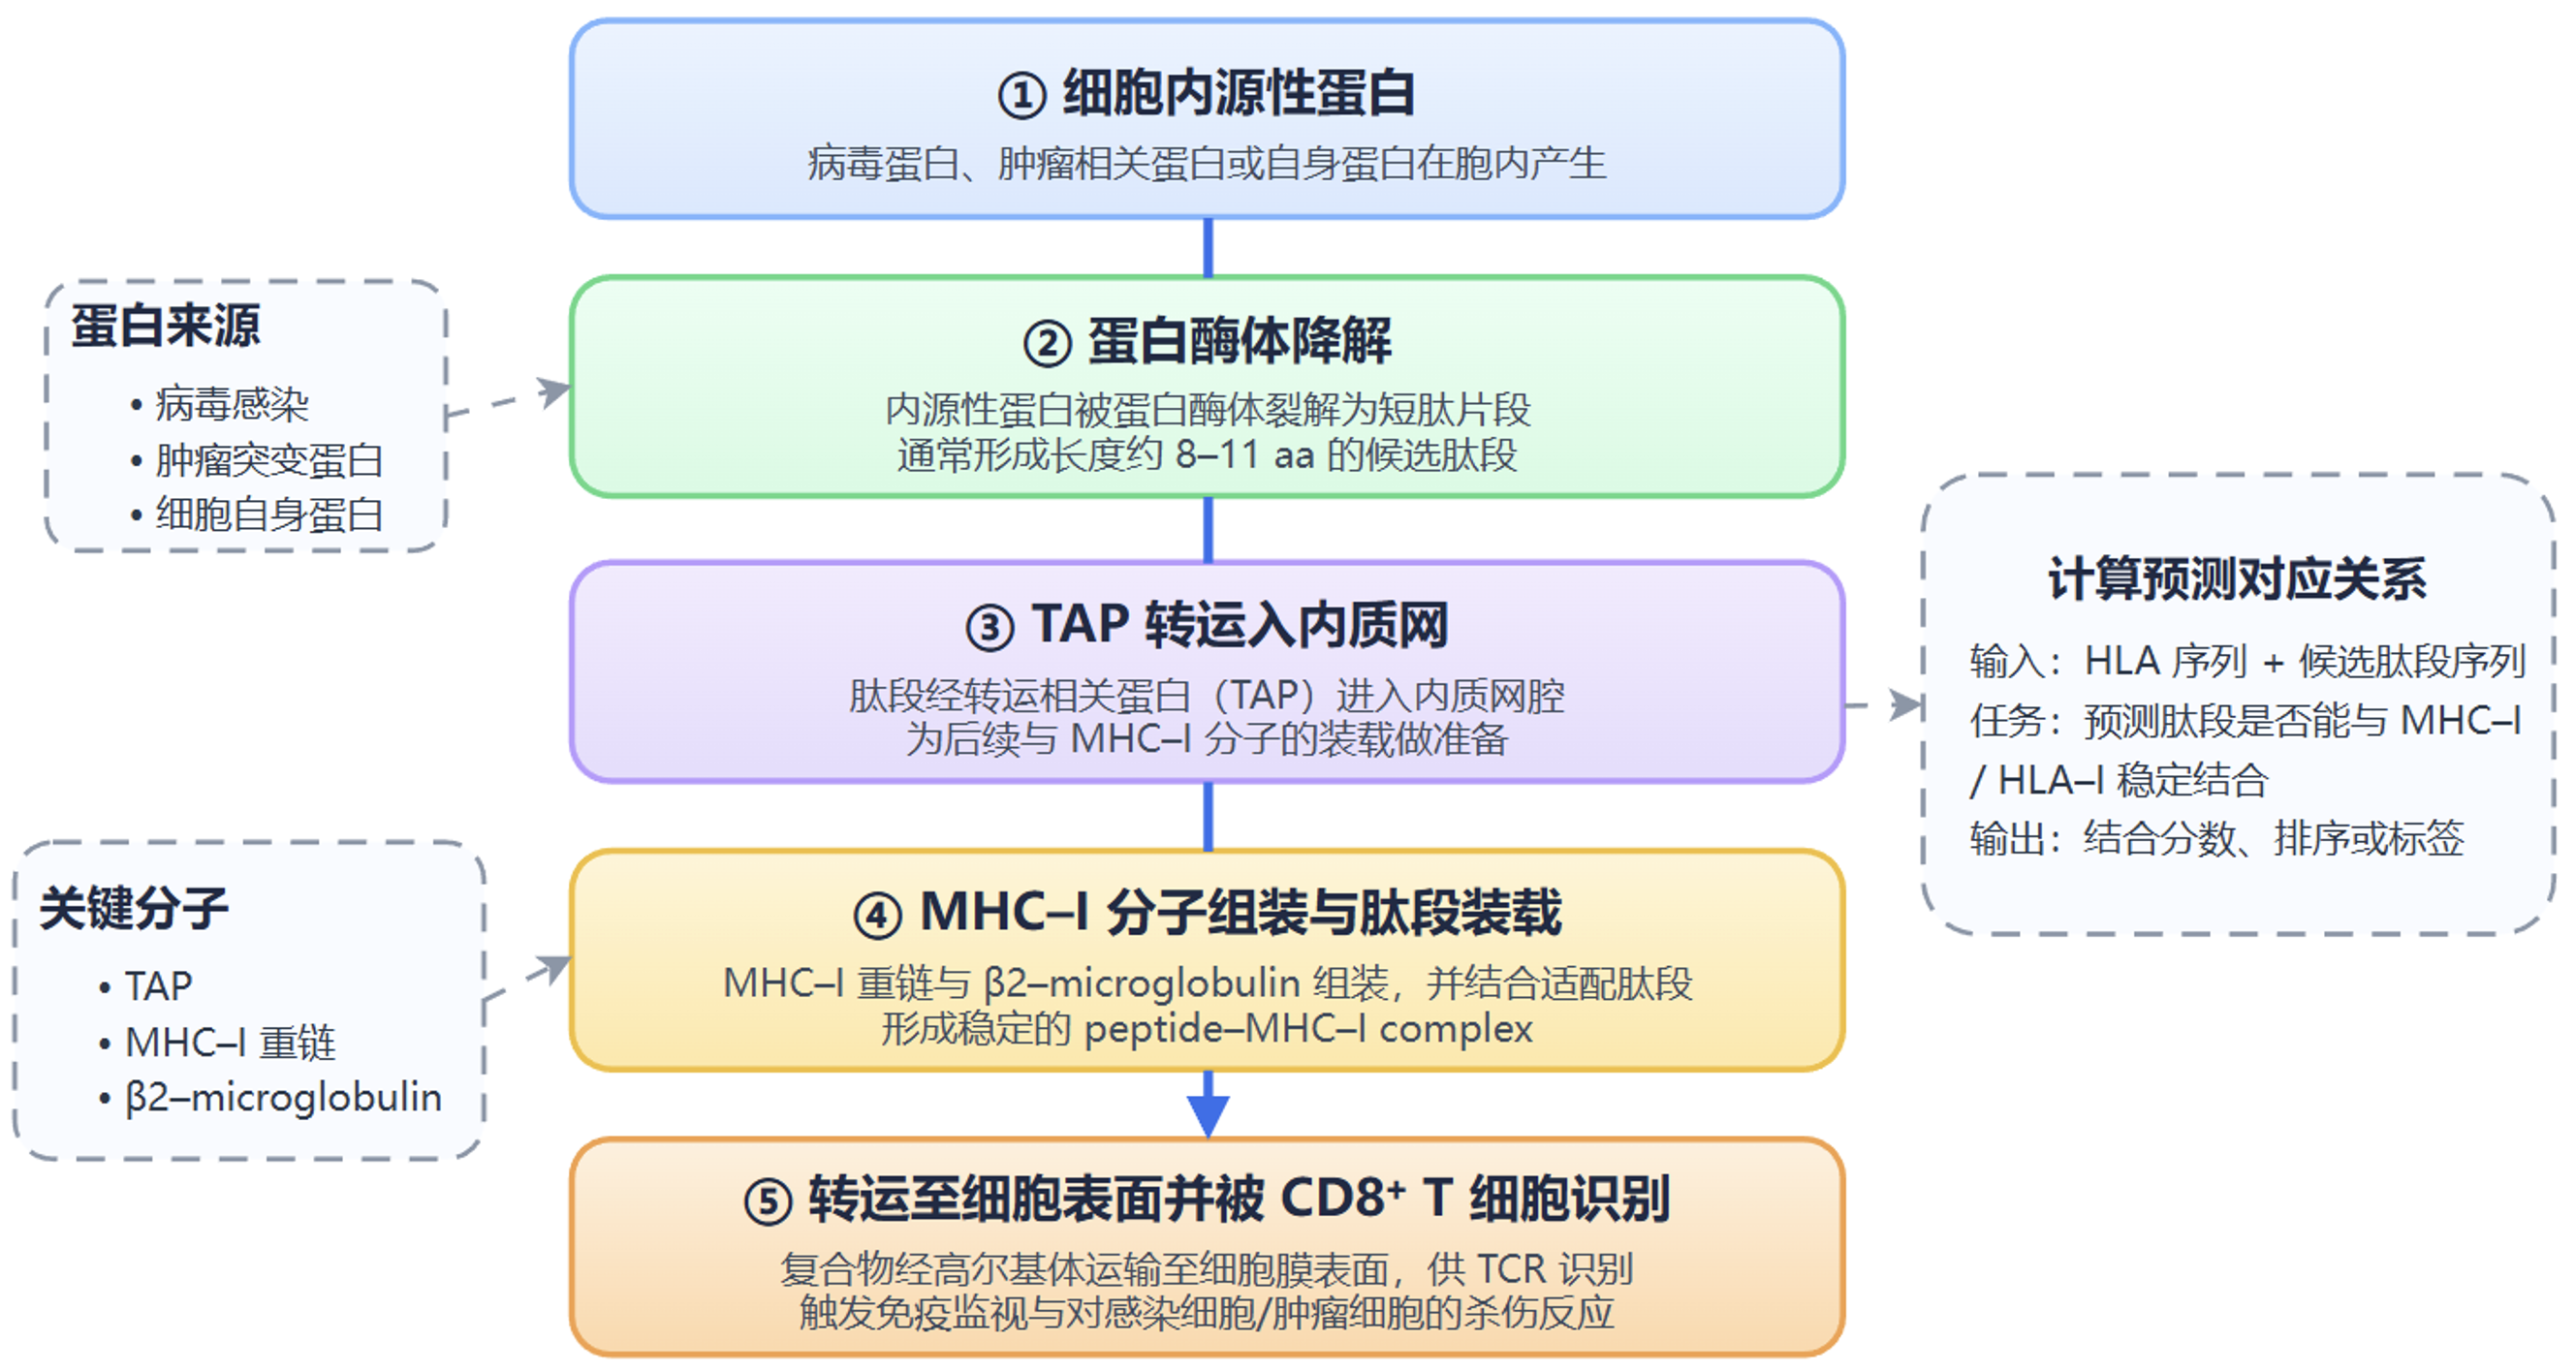
\includegraphics[width=0.85\textwidth]{figures/MHC-I-抗原递呈过程示意图.png}
    \caption{MHC-I 抗原递呈过程示意图}
    \label{fig:MHC-Peptide}
\end{figure}

\subsection{HLA等位基因多态性与预测难点}

MHC-I 肽段结合预测的挑战首先来自 HLA 分子的高度多态性。不同等位基因在结合槽结构、关键氨基酸位点和理化性质上的差异，导致其各自具有不同的肽段锚定位点偏好和长度分布偏好。这意味着同一条肽段在不同 HLA 背景下可呈现完全不同的结合能力，而同一 HLA 分子对长度、组成各异的肽段也具有选择性。

其次，肽段序列的表示本身具有复杂性。虽然 MHC-I 结合肽通常长度较短，但其局部氨基酸组合、位置依赖关系以及与 HLA 结合槽的匹配模式并非简单的线性关系。依赖结合基序、位置特异性打分矩阵或浅层机器学习的方法，在复杂等位基因背景和大规模候选肽段面前，表达能力和泛化能力往往受限。

最后，真实应用场景中的预测任务通常不是对少量候选肽段进行二分类判断，而是需要在大规模候选空间中快速筛选与排序。因此，一个具有实际应用价值的模型不能仅追求预测精度，还必须兼顾计算效率、存储成本和部署可行性。

\subsection{免疫多肽结合预测的任务形式}

从建模角度看，MHC-I 肽段结合预测常见的任务形式主要有两类。第一类是分类或回归式预测，即直接判断结合或估计结合强度。第二类是表示学习式预测，将 HLA 与肽段分别映射至统一向量空间，通过距离或相似度完成匹配、排序和检索。

与传统分类框架相比，表示学习式方法不仅能完成结合预测，还能天然支持大规模候选肽段筛选、向量检索和下游数据库缩减，因此在需要处理海量候选肽段的工程场景中扩展性更强。

本课题研究的 FennOmix.MHC 属于表示学习式方法。该模型以 HLA/MHC-I 蛋白序列和候选肽段序列作为两个模态输入，分别编码为向量，并在共享嵌入空间中通过距离关系刻画两者的匹配程度，从而实现结合预测和候选筛选。

\section{FennOmix.MHC模型与表示学习基础}

\subsection{FennOmix.MHC基础框架}

FennOmix.MHC 是面向 MHC-I 肽段结合预测的深度学习模型，其核心是将 HLA/MHC-I 蛋白序列与候选肽段序列视为两个模态，分别编码至共享嵌入空间。在该空间中，真实结合的 HLA–肽段样本对彼此靠近，而非结合或随机配对样本则相互远离。

相比于直接建模为分类任务，双编码器加共享空间的设计具有两方面优势。其一，模型可分别学习 HLA 与肽段的序列表示，再通过统一度量完成匹配，有助于增强对不同等位基因和不同肽段分布的泛化能力。其二，共享嵌入空间天然适合候选肽段检索、相似度排序和缩库辅助搜库等任务，因而更契合大规模工程应用场景。

\begin{figure}
    \centering
    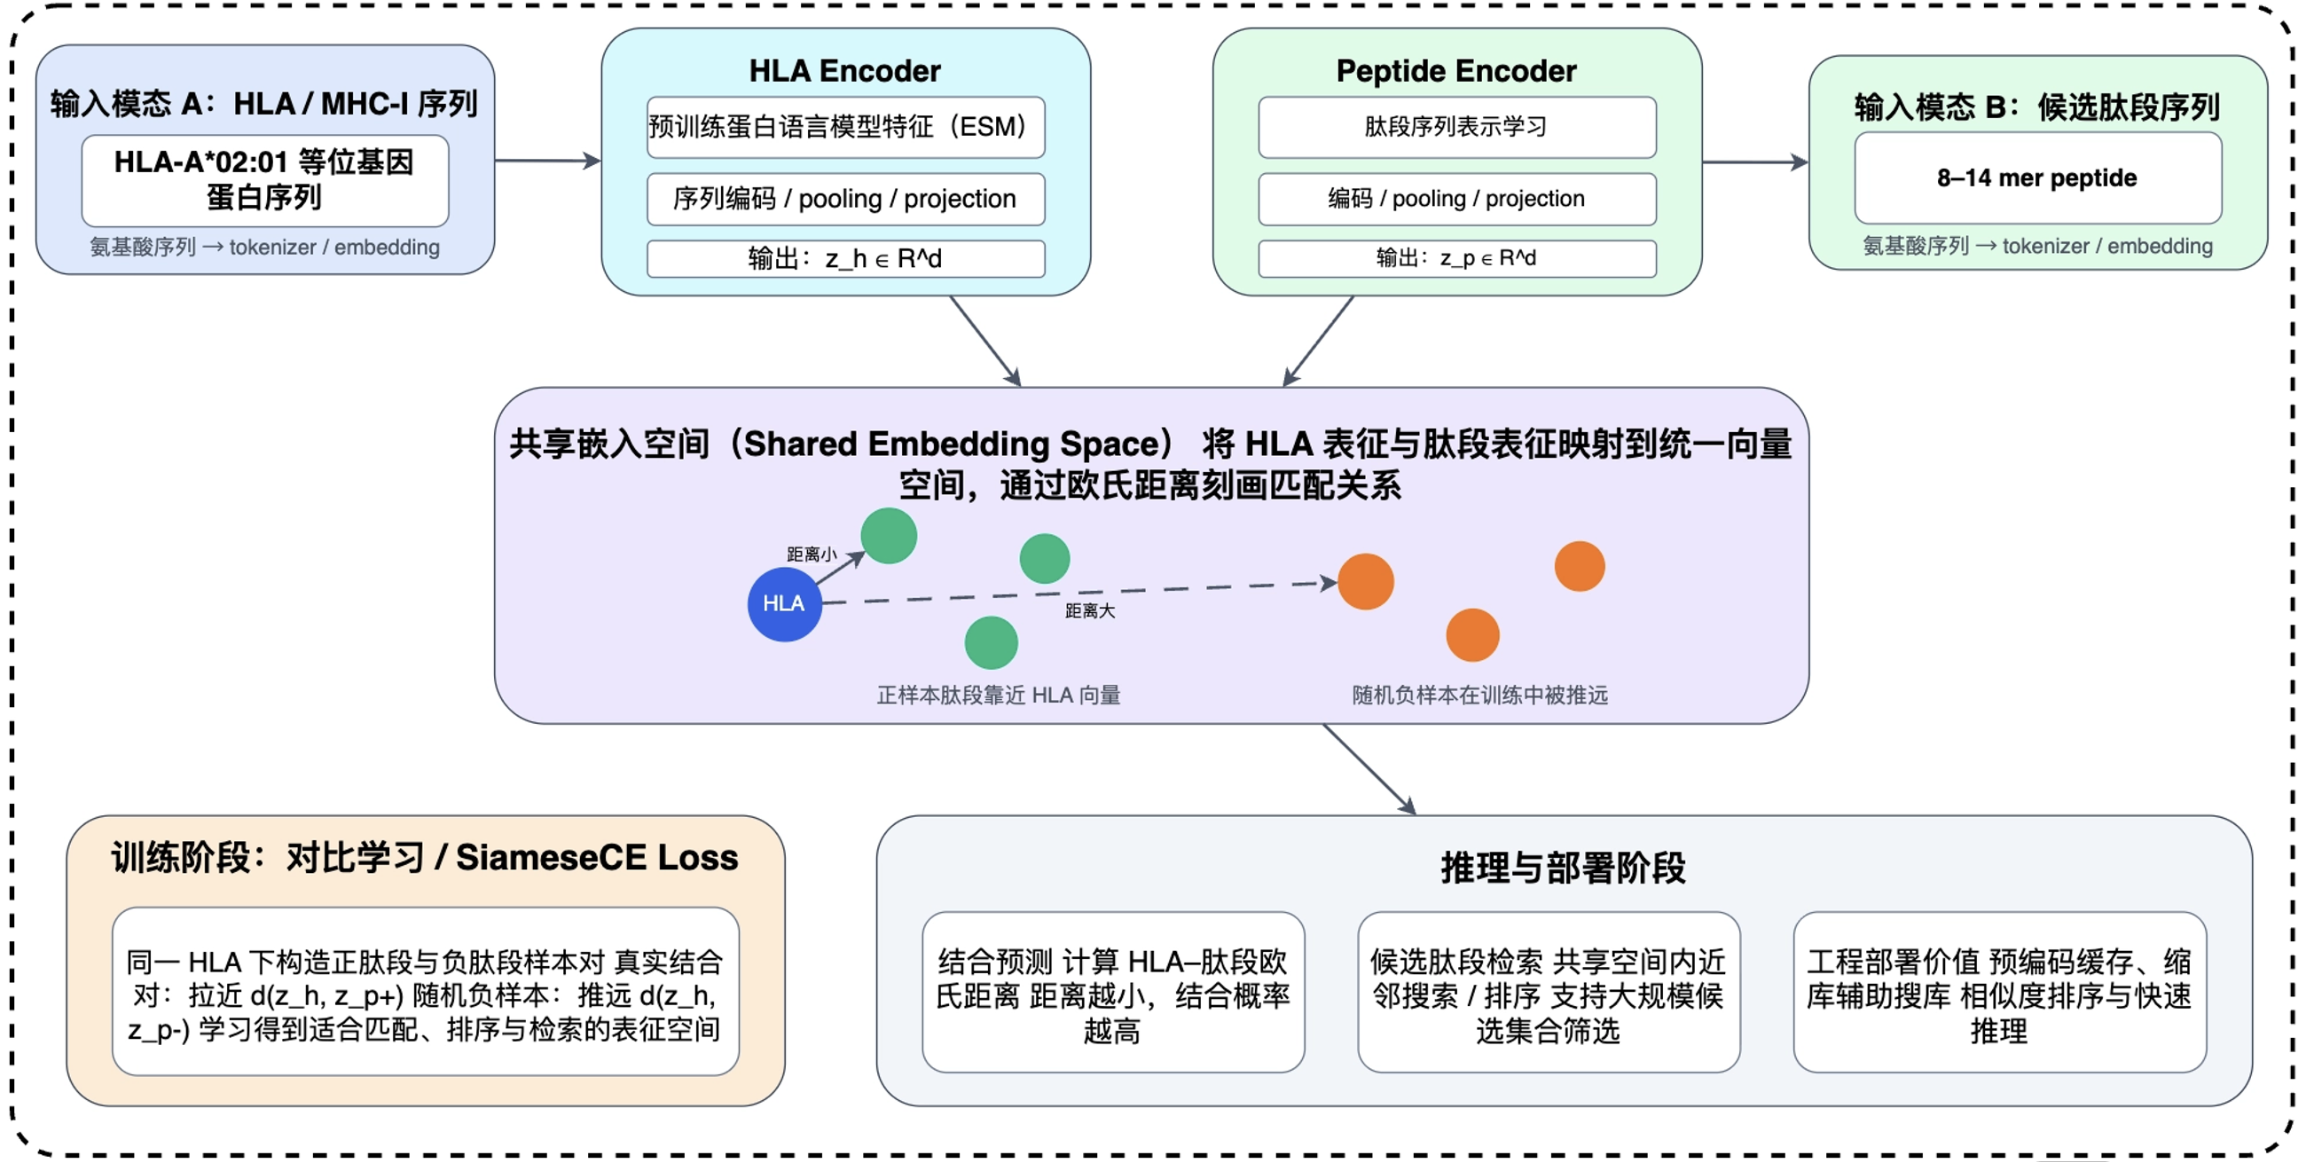
\includegraphics[width=1.0\textwidth]{figures/FennOmix.MHC 基础框架图.png}
    \caption{FennOmix.MHC 基础框架图}
    \label{fig:fennomixmhc-framework} 
\end{figure}

\subsection{输入表示与双模态编码}

FennOmix.MHC 的输入包含两部分：HLA/MHC-I 蛋白序列与候选肽段序列。模型将这两类氨基酸序列编码为向量，供后续相似度计算与匹配预测使用。在后续降维设计中，HLA 编码器以 ESM2 产生的 480 维 token 表示作为上游输入，并进一步通过线性映射或 MLP 进行维度压缩，可见该模型的基础编码阶段已具备较强的预训练表示背景。

从表示学习角度看，双模态编码的本质是在两个输入空间分别提取结构与语义特征，并将其映射至统一语义空间。对 HLA 分子而言，模型需捕获其结合槽相关的序列特征；对肽段而言，则需学习与锚定位点、长度偏好和整体结合模式相关的表示。二者共同决定了后续距离度量的有效性。

\subsection{对比学习与嵌入空间度量}

对比学习的核心在于通过构造正样本对与负样本对，学习一个能够在表示空间中区分它们的映射函数。理想情况下，正样本对在空间中彼此靠近，负样本对则相互远离。在 MHC-I 肽段结合预测任务中，可把真实结合的 HLA–肽段组合视为正样本对，随机配对或 decoy 构造视为负样本对。

与传统监督分类不同，对比学习更关注样本间的相对关系，而非类别标签本身。这种特性使其尤其适合匹配、检索和排序类任务。在很多实际场景中，模型最终并不需要只输出“结合”或“不结合”，而是要在大量候选肽段中给出可靠的相对优先级排序。由对比学习构建的嵌入空间，恰好能够天然支撑这类需求。

共享嵌入空间采用欧氏距离衡量 HLA 与肽段嵌入的匹配程度。肽段嵌入与目标 HLA 嵌入之间的欧氏距离越小，表明该肽段越有可能属于该 HLA 的潜在结合肽段；距离越大，匹配可能性越低。

从表示学习角度看，一个有效的嵌入空间不仅要求正负样本可分，还要求空间结构具备较好的稳定性。当模型经历降维、剪枝或量化等优化操作后，如果向量邻域关系仍能基本保持，就说明原始语义空间没有发生明显扭曲。因此，评价嵌入空间结构是否稳定，是本文后续模型轻量化和缓存压缩研究的重要依据。

\section{评价指标与下游检索任务}

\subsection{基于排名阈值的召回率}

基于排名阈值的召回率用于考察真实结合肽段能否进入模型排序结果的前列。本文使用 rank@0.1、rank@0.5 和 rank@2.0 三个指标，分别统计真实阳性样本出现在预测排名前 0.1\%、0.5\% 和 2.0\% 候选中的比例。

设测试集中 HLA 等位基因集合为 $H$。对于某一等位基因 $h \in H$，其候选肽段集合记为 $C_h$，真实结合肽段集合记为 $P_h$。模型对 HLA 嵌入与肽段嵌入计算欧氏距离，距离越小代表模型判定该肽段与该 HLA 结合的可能性越大。肽段 $p$ 与 HLA $h$ 的距离为：
\begin{equation}
    d(h,p)=\left\|z_h-z_p\right\|_2
\end{equation}
其中，$z_h$ 和 $z_p$ 分别为 HLA 和肽段的嵌入向量。

对所有候选肽段按距离从小到大排序后，肽段 $p$ 在候选集合 $C_h$ 中的排名可表示为：
\begin{equation}
\operatorname{rank}_h(p)
=
1+
\sum_{q \in C_h}
\mathbb{I}\left(d(h,q)<d(h,p)\right)
\end{equation}
式中，$\mathbb{I}(\cdot)$ 为指示函数，条件成立时取值为 1，否则取值为 0。

给定排名比例阈值 $\alpha$，且 $\alpha \in \{0.001,0.005,0.02\}$，分别对应 rank@0.1、rank@0.5 和 rank@2.0，可保留的候选肽段数量为：
\begin{equation}
K_h(\alpha)=\left\lceil \alpha |C_h| \right\rceil
\end{equation}

则基于排名阈值的召回率定义为：
\begin{equation}
\operatorname{Recall}_{\operatorname{rank}@\alpha}
=
\frac{
\sum_{h \in H}
\sum_{p \in P_h}
\mathbb{I}\left(
\operatorname{rank}_h(p) \le K_h(\alpha)
\right)
}{
\sum_{h \in H}|P_h|
}
\end{equation}
其中，分子表示所有真实结合肽段中被排入前 $\alpha$ 比例候选集合的样本数，分母为测试集真实结合肽段总数。该指标越高，说明模型越能将真实结合肽段排在候选列表前部。

这类指标更关注模型在大规模候选筛选中的优先级排序能力，而非简单的二分类准确率。在实际应用中，研究者通常希望模型将真实结合肽段置于候选列表前部，以便优先进行实验验证或数据库检索。因此，rank-recall 能较好地反映模型在候选筛选场景中的实用价值。

\subsection{基于距离阈值的召回率}

基于距离阈值的召回率用于评价真实结合样本在共享嵌入空间中的邻域聚集程度。本文采用 dist@0.2、dist@0.3 和 dist@0.4 三个指标，统计真实结合肽段与对应 HLA 嵌入之间欧氏距离不超过给定阈值的比例。

共享嵌入空间中，HLA 与肽段的匹配程度由欧氏距离度量。对 HLA $h$ 及其真实结合肽段 $p$，二者距离为：
\[
d(h,p)
=
\left\|z_h-z_p\right\|_2
=
\sqrt{
\sum_{j=1}^{D}
\left(z_{h,j}-z_{p,j}\right)^2
}
\]
其中 $D$ 为嵌入向量维度，$z_{h,j}$ 和 $z_{p,j}$ 分别表示 HLA 嵌入和肽段嵌入在第 $j$ 个维度上的取值。

对于给定距离阈值 $\tau$，其中 $\tau \in \{0.2,0.3,0.4\}$，基于距离阈值的召回率定义为：
\begin{equation}
\operatorname{Recall}_{\operatorname{dist}@\tau}
=
\frac{
\sum_{h \in H}
\sum_{p \in P_h}
\mathbb{I}\left(d(h,p)\le \tau\right)
}{
\sum_{h \in H}|P_h|
}
\end{equation}
分子为所有真实结合肽段中与对应 HLA 嵌入距离不超过 $\tau$ 的样本数，分母为真实结合肽段总数。$\operatorname{Recall}_{\operatorname{dist}@\tau}$ 较高时，说明更多真实结合肽段被映射到对应 HLA 周围较近的邻域内，模型学习到的共享嵌入空间具有较好的聚集性。

与 rank-recall 不同，distance-recall 更关注嵌入空间本身的几何结构，它不判断真实阳性样本是否位于排序结果的前若干比例，而是考察它们是否聚集在目标 HLA 附近的邻域中。因此，该指标适合分析降维、剪枝或量化等操作是否破坏了原始嵌入空间结构。若模型压缩后 distance-recall 仍保持稳定，则说明轻量化操作对 HLA-肽段匹配空间的扰动较小，模型仍适用于后续候选筛选与检索任务。

\subsection{缩库辅助搜库与Overlap评价}

单一指标很难全面评价模型表现。仅观察 rank-recall 容易偏向候选排序能力，忽略空间结构是否稳定；仅关注 distance-recall 则可能无法充分反映模型在大规模候选优先级排序中的实际效果。

为此，本文联合使用排名类与距离类指标，同时考察模型的候选筛选能力和空间结构保持能力。只有当模型在多个评价维度上均表现稳定时，才能说明其既具备较好的预测质量，又拥有进一步部署应用的基础。

\label{sec:direct-model-search}

在真实质谱鉴定中，数据库检索通常将实验 MS/MS 谱图与候选肽段库进行匹配，获得 PSM、肽段及蛋白层面的鉴定结果。免疫多肽组学的候选空间往往极为庞大，直接在完整库上检索不仅计算开销大，还可能引入无关候选带来的匹配噪声。

因此，在保持鉴定覆盖度的前提下尽可能压缩候选空间，是提升检索效率的关键。对于 MHC-I 肽段结合预测模型而言，若能提前筛选出更可能与特定 HLA 结合的候选肽段，就有可能为下游数据库检索提供一个更精简、更具针对性的候选库。

为衡量模型在真实质谱鉴定场景中的实际价值，本文对比 Direct Search 与 Model-assisted Search 两种流程。

Direct Search 作为基线流程，在已知等位基因条件下直接对原始候选数据库进行检索，不依赖模型预筛选，可为后续比较提供参照。

Model-assisted Search 则是模型辅助缩库流程，先利用 MHC-I 肽段结合预测模型对候选肽段进行打分或筛选，构建等位基因特异的缩减数据库，再在该缩减库上执行检索。其核心思路是通过模型先验收窄候选空间，以提升检索效率或增强候选库的针对性。

两种流程的关键区别在于 Model-assisted Search 在检索之前增加了模型筛选步骤。若缩库流程能在更小的候选规模下保持对基线结果的高覆盖，就说明模型拥有较好的下游应用价值。

在缩库辅助搜库的下游任务中，本文对 Direct Search 与 Model-assisted Search 得到的肽段级结果进行 overlap 分析。记 Direct Search 检出的肽段集合为 $S_D$，Model-assisted Search 检出的肽段集合为 $S_M$，二者交集为：$S_I = S_D \cap S_M$，$S_I$ 表示两种流程共同检出的肽段。基于这三个集合，采用以下六项指标评估缩库效果。

Precision-like 反映缩库结果中与基线一致的肽段占比，定义为：
\begin{equation}
\mathrm{Precision}\mbox{-}\mathrm{like}
=
\frac{|S_I|}{|S_M|}
\end{equation}
Recall-like 反映缩库流程对基线结果的保留程度，定义为：
\begin{equation}
\mathrm{Recall}\mbox{-}\mathrm{like}
=
\frac{|S_I|}{|S_D|}
\end{equation}
Overlap-F1 综合 Precision-like 与 Recall-like，整体衡量两类结果的吻合度：
\begin{equation}
\mathrm{Overlap}\mbox{-}\mathrm{F1}
=
\frac{
2 \times
\mathrm{Precision}\mbox{-}\mathrm{like}
\times
\mathrm{Recall}\mbox{-}\mathrm{like}
}{
\mathrm{Precision}\mbox{-}\mathrm{like}
+
\mathrm{Recall}\mbox{-}\mathrm{like}
}
\end{equation}
Loss Rate 衡量 Direct Search 结果中被缩库流程遗漏的肽段比例：
\begin{equation}
\mathrm{Loss}\ \mathrm{Rate}
    =
    \frac{\left|S_D - S_M\right|}{\left|S_D\right|}
\end{equation}
Expansion Rate 衡量 Model-assisted Search 相对于 Direct Search 新增肽段的比例：
\begin{equation}
\mathrm{Expansion}\ \mathrm{Rate}
    =
    \frac{\left|S_M - S_D\right|}{\left|S_D\right|}
\end{equation}
Comprehensive Score（CS）用于综合评价缩库流程的整体表现，定义为：
\begin{equation}
\mathrm{CS}
    =
\frac{1}{3}
\left(
\mathrm{Overlap}\mbox{-}\mathrm{F1}
+
\left(1-\mathrm{Loss}\ \mathrm{Rate}\right)
+
\frac{1}{1+\mathrm{Expansion}\ \mathrm{Rate}}
    \right)
\end{equation}
在上述指标中，Precision-like、Recall-like、Overlap-F1 和 CS 越高，说明缩库结果与基线的吻合度越好；Loss Rate 和 Expansion Rate 越低，则意味着缩库引起的肽段丢失和新引入差异越少。这些指标从重合度、基线保留率、遗漏程度和新增差异等维度，综合评价模型辅助缩库流程的实际效果。

对于本研究而言，缩库辅助搜库并不是一项附加实验，而是连接模型性能与实际应用价值的关键桥梁。一方面，模型在 rank-recall 和 distance-recall 上的好成绩，未必能直接转化为真实数据库检索中的贡献；另一方面，如果模型经过降维、剪枝或缓存压缩后，仍能在缩库辅助搜库中保持较高的覆盖度和综合评分，就表明它既“测得好”，也“用得上”。因此，我们将缩库辅助搜库任务作为后续实验分析的重要环节，用于检验不同轻量化方案在真实质谱鉴定场景中的实际效果。特别是在比较不同的 64 维降维模型时，除常规的 rank-recall 和 distance-recall 外，还会结合 Direct Search 与 Model-assisted Search 的肽段重叠结果，从多指标角度进行综合评价。相关实验与结论将在第三章给出。

\section{面向部署的模型轻量化方法设计}

\subsection{原始模型部署瓶颈与轻量化思路}

FennOmix.MHC 通过共享嵌入空间对 HLA 分子与候选肽段进行联合建模，其基本输出是 embedding 向量。高维向量虽有利于捕获更丰富的序列语义，但部署时这种高维表示会直接演变为沉重的缓存存储负担。

\begin{figure}[htbp]
    \centering
    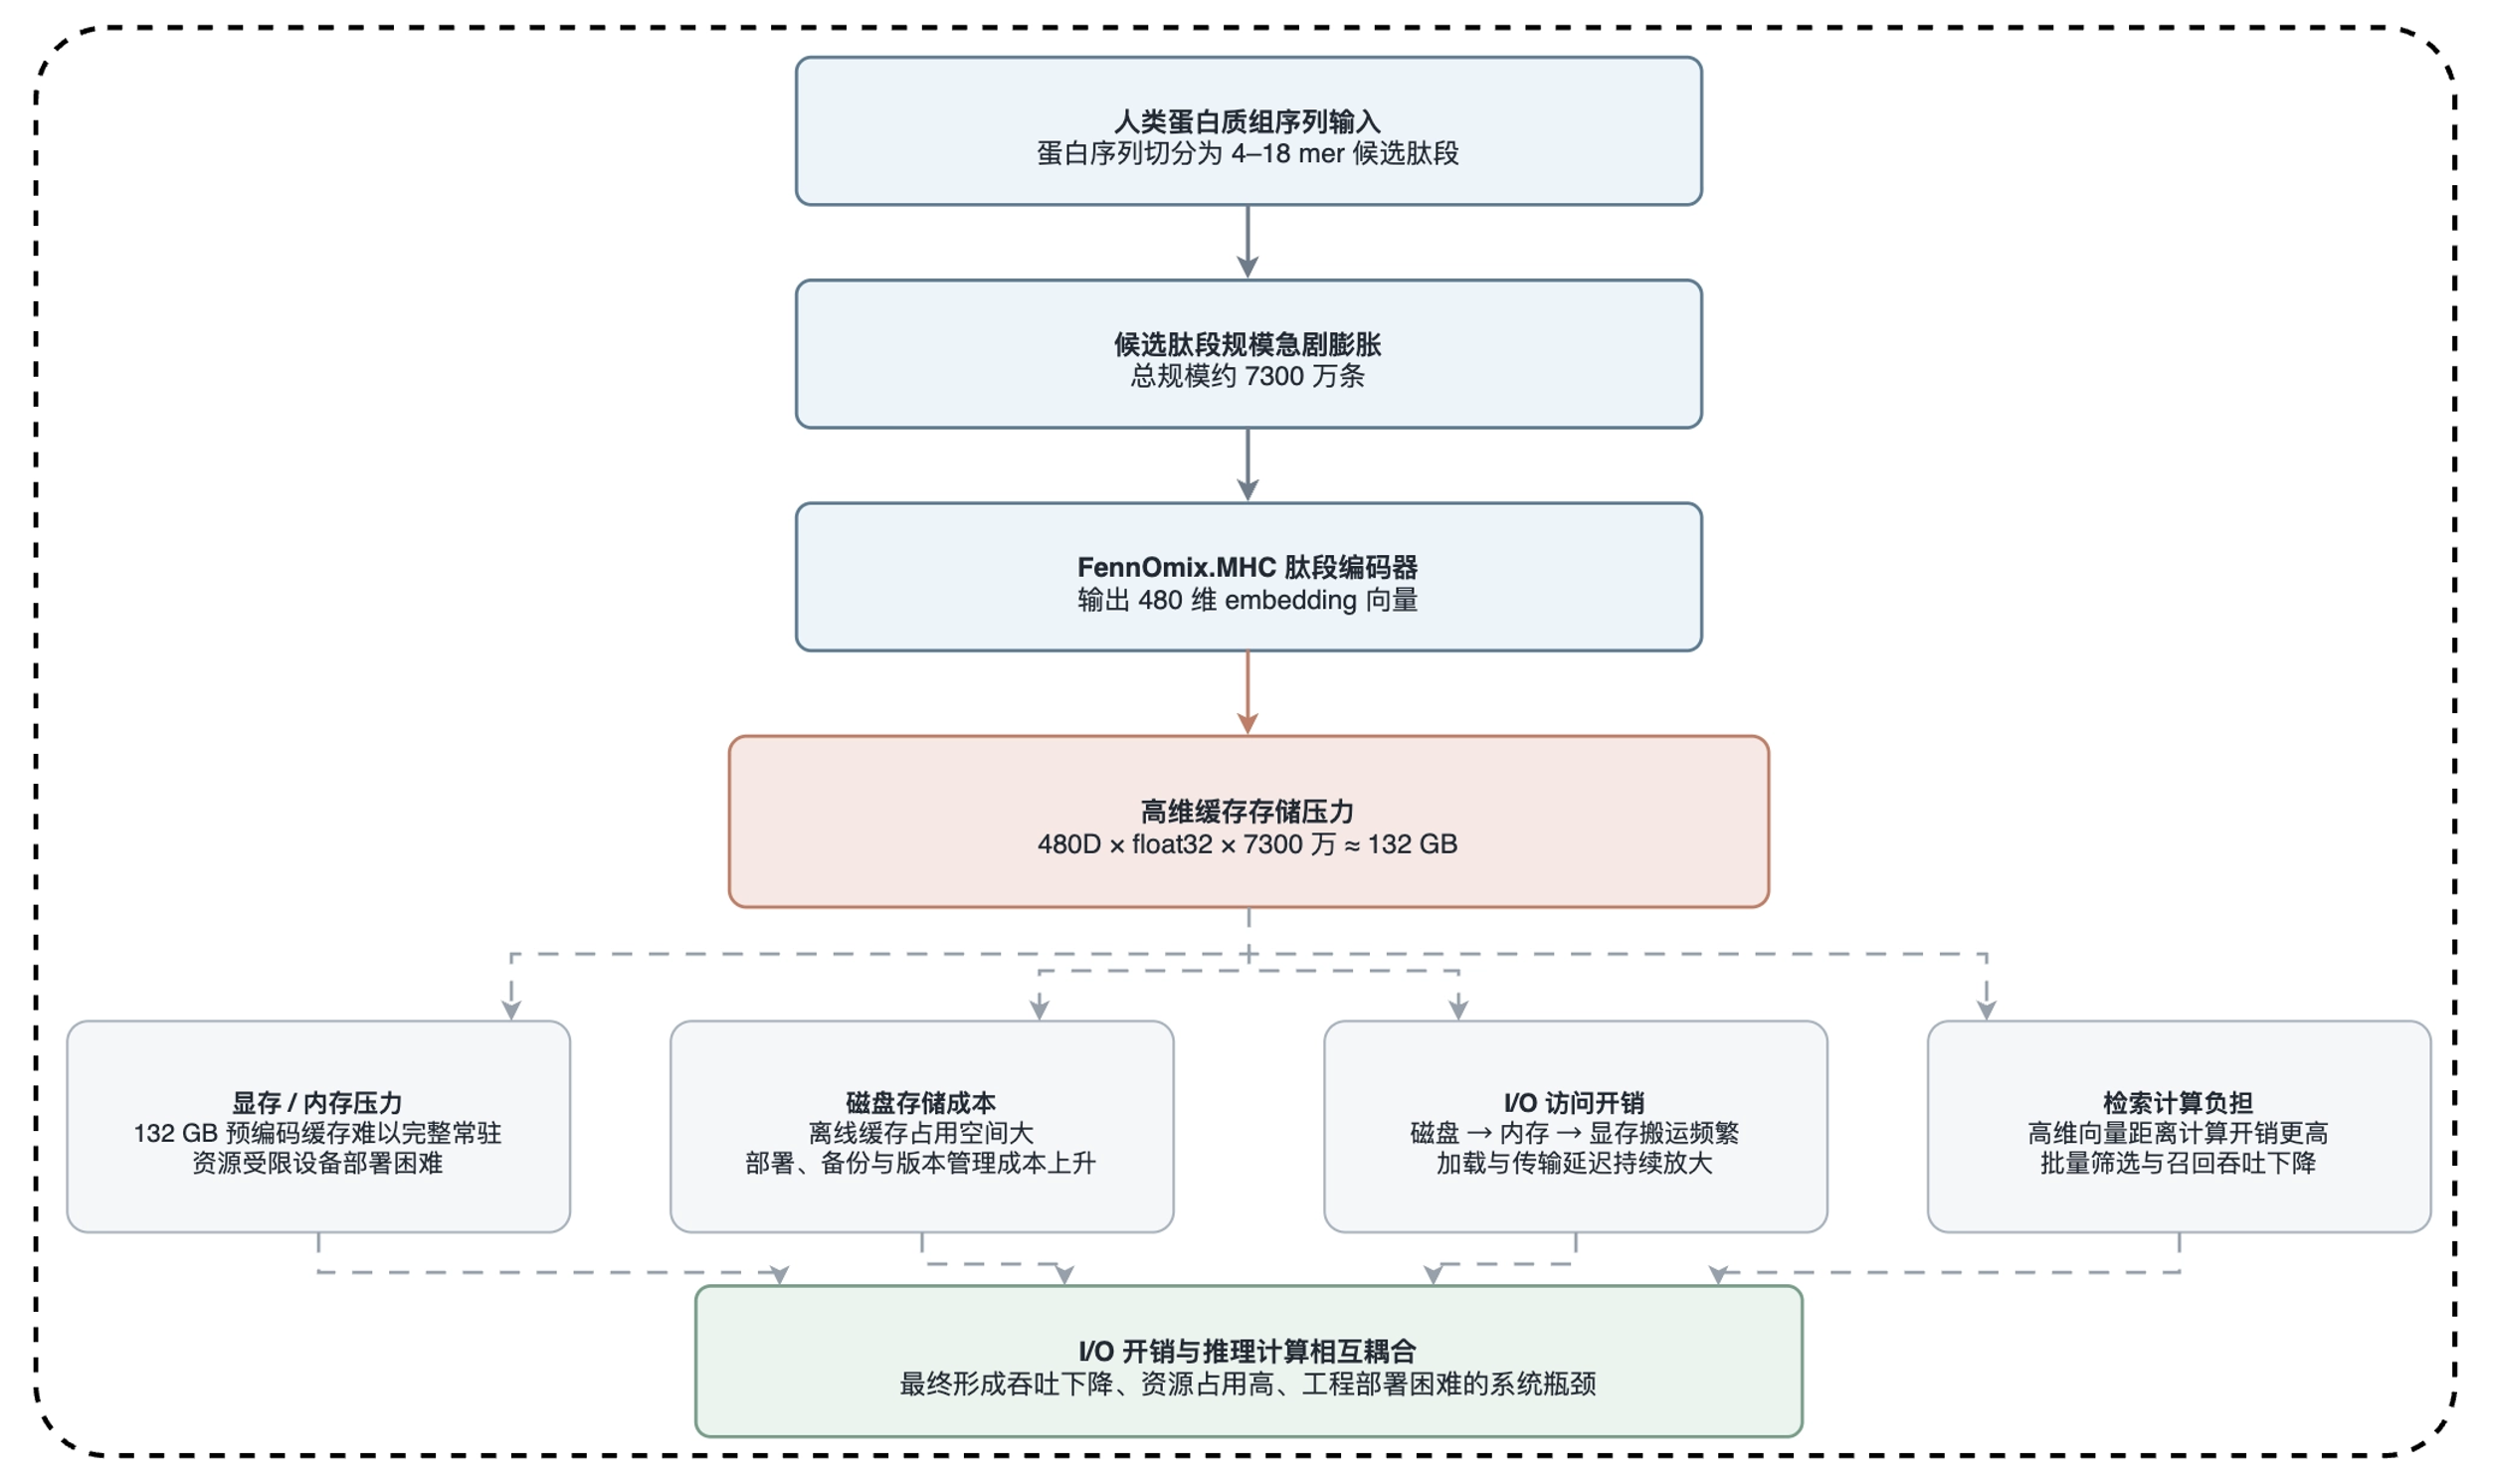
\includegraphics[width=1.0\textwidth]{figures/fig4_bottleneck.png}
    \caption{原始模型部署瓶颈示意图}
    \label{fig:original-model-bottleneck}
\end{figure}

在大规模人类蛋白质组应用中，蛋白质序列会被切割成海量候选肽段，每条肽段均需生成向量表示。如果仍沿用原始的 float32 高维向量进行离线缓存，缓存文件将占用大量存储空间，很难整体驻留在单块 GPU 显存或普通主机内存中，同时还会加重磁盘开销、文件传输、版本管理与部署备份等成本。从工程角度看，肽段缓存过大不仅意味着静态存储成本居高不下，还会拖慢后续模型调用中的读取、加载和数据搬运效率。特别是当候选肽段需要频繁参与距离计算时，缓存规模直接制约着系统响应速度和部署便捷性。因此，压缩肽段 embedding 维度是缓解大规模缓存压力的核心切入点。

原始模型的部署压力并非单纯来自参数量，而是高维向量表示、缓存机制和检索流程相互耦合的结果。维度越高，单次距离计算和批量检索的计算开销越大；缓存越大，数据从磁盘到内存、从内存到显存的搬运成本也越高。系统需要在大规模候选肽段中执行批量筛选时，I/O 延迟与向量计算相互叠加，最终拉低整体吞吐效率。

此外，模型结构本身也可能存在冗余。对于采用 Transformer 结构的编码器，不同注意力头、前馈网络隐藏单元以及不同层模块对最终表示的贡献并不均匀。若不加区分地全部保留，会引入不必要的计算消耗。因此，部署优化不能只盯着输出向量维度，还必须分析模型内部是否存在可压缩的空间。

针对上述瓶颈，我们将 FennOmix.MHC 的模型轻量化优化划分为两个方向：表示压缩与结构压缩。

表示压缩主要回应大规模肽段缓存的压力。通过缩减模型输出 embedding 维度，可以直接降低肽段向量的离线存储开销，并减少后续距离计算和检索过程的时间、空间消耗。对于规模庞大的候选肽段库而言，表示压缩是提升系统可部署性的基础。结构压缩则回应模型推理阶段的冗余计算问题。通过分析 Transformer 编码器中不同注意力头和前馈网络单元的重要性，可以识别贡献较低的组件，进而评估剪枝的可行性。两种压缩并非替代关系，而是互为补充：表示压缩侧重削减输出表示及缓存带来的系统成本，结构压缩则压缩模型内部的计算开销。

基于这一思路，本章将依次介绍编码维度压缩设计、线性和非线性降维方案的构建，以及基于重要性分析的结构剪枝方法。这些方法的具体实验效果将在第三章进行验证。

\subsection{编码维度压缩设计}

编码降维是本文面向部署优化的第一步，其核心并非单纯压缩向量维度，而是在守住 MHC-I 肽段结合预测能力和嵌入空间结构稳定性的前提下，显著削减肽段预编码缓存的存储成本。FennOmix.MHC 后续的大规模候选筛选、距离排序以及下游缩库辅助搜库，都依赖于 embedding 空间的几何关系。因此，一个合理的降维方案需同时满足以下三点：第一，候选排序能力保持基本稳定，降维后的模型仍能将真实结合肽段排在候选列表前部；第二，嵌入空间的邻域结构尽量得到保留，真实结合肽段仍聚集在对应 HLA 表示附近；第三，缓存体积明显下降，体现出工程价值。

这实际上是将输出维度压缩定位为“预测性能—空间结构—存储成本”三者的权衡，而不是一味追求最低维度。为考察不同输出维度对模型性能和缓存成本的影响，我们设置了多组输出维度方案，包括原始高维表示和若干低维压缩表示，以此观察维度逐步降低时，性能、结构稳定性和缓存成本之间的变化关系。

评价方面，我们联合使用两类指标：基于排名阈值的 rank-recall，评估模型在大规模候选筛选中的排序能力；基于欧氏距离阈值的 distance-recall，评估真实结合样本在共享嵌入空间中的邻域聚集程度。它们分别对应“候选排序能力”和“空间结构保持性”，可以从不同侧面反映降维带来的影响。缓存成本则通过 $S = N \times D \times B$ （其中， $N$ 是候选肽段数量，$D$ 是向量维度，$B$ 是每个元素占用字节）估算，在候选肽段数量和数据类型固定的条件下，缓存规模与输出维度近似线性相关，降低维度能直接缩减缓存体积。

在输出维度的选取上，最低维度并不是唯一目标。维度过高，缓存和计算成本依然偏高；维度过低，则可能破坏嵌入空间结构，损害候选排序和后续检索效果。因此，合理的维度应在性能保持与成本降低之间找到平衡。我们主要依据以下原则来选择后续重点优化的方案：优先确保嵌入空间结构稳定，distance-recall 是判断降维可接受的重要依据；兼顾候选排序能力，尽可能维持较好的 rank-recall；关注缓存压缩带来的实际收益，若某维度方案在性能下降可控的同时显著缩减缓存，则更适合作为后续缓存压缩、索引检索和系统部署的基础。第三章将对不同维度方案进行系统的实验比较，并据此确定适用于后续部署优化的默认输出维度。

\subsection{线性与非线性降维方案设计}

在输出维度压缩的基础上，还需比较相同维度条件下不同映射结构对模型性能和部署成本的影响。为此，我们设计了线性降维和非线性降维两类方案：线性降维采用单层线性映射，将上游编码结果直接投影到目标低维空间；非线性降维采用包含隐藏层和激活函数的 MLP 结构。线性方案结构简单、参数量少，易于训练和部署；MLP 表达力更强，但会引入额外的参数和计算开销。

实验中构建了两个 64 维低维模型进行对照：MHC-64D-BertLinear 和 MHC-64D-BertMLP，在输出维度一致的条件下比较，保证差异主要来源于映射结构本身。

首先采用常规的 rank-recall 和 distance-recall 评估两类模型的基础预测能力。若两者在常规指标上表现接近，单靠这些指标不足以做出取舍，还需要结合下游任务和模型复杂度进一步判断。为此，我们进一步引入缩库辅助数据库检索任务。模型先根据目标 HLA 对候选肽段进行筛选，构建等位基因特异的缩减数据库，再将这一缩库结果与直接检索流程进行肽段重叠比较。评价采用 Precision-like、Recall-like、Overlap-F1、Loss Rate、Expansion Rate 和 Comprehensive Score 等指标，从覆盖度、一致性、结果丢失和新增差异等角度衡量缩库效果。将 Linear 和 MLP 两类模型嵌入相同的下游流程进行比较，能更真实地反映不同降维结构在实际应用场景中的适用程度。

最终默认降维模型的选定需要综合三方面因素：常规预测性能应在 rank-recall 和 distance-recall 上保持相对稳定，表明候选排序和空间结构未受明显冲击；下游缩库辅助搜库任务中应保持较好的覆盖度和一致性，体现其在实际流程中的价值；同时优先选择工程部署成本更低的方案。若 Linear 与 MLP 的性能差别不大，则结构更轻量、参数更少、实现更简单的 Linear 更适合作为默认部署模型。第三章将结合常规指标与下游缩库辅助搜库结果，对两类降维模型进行全面比较，并确定后续系统优化所采用的默认模型。

\begin{figure}[htbp]
    \centering
    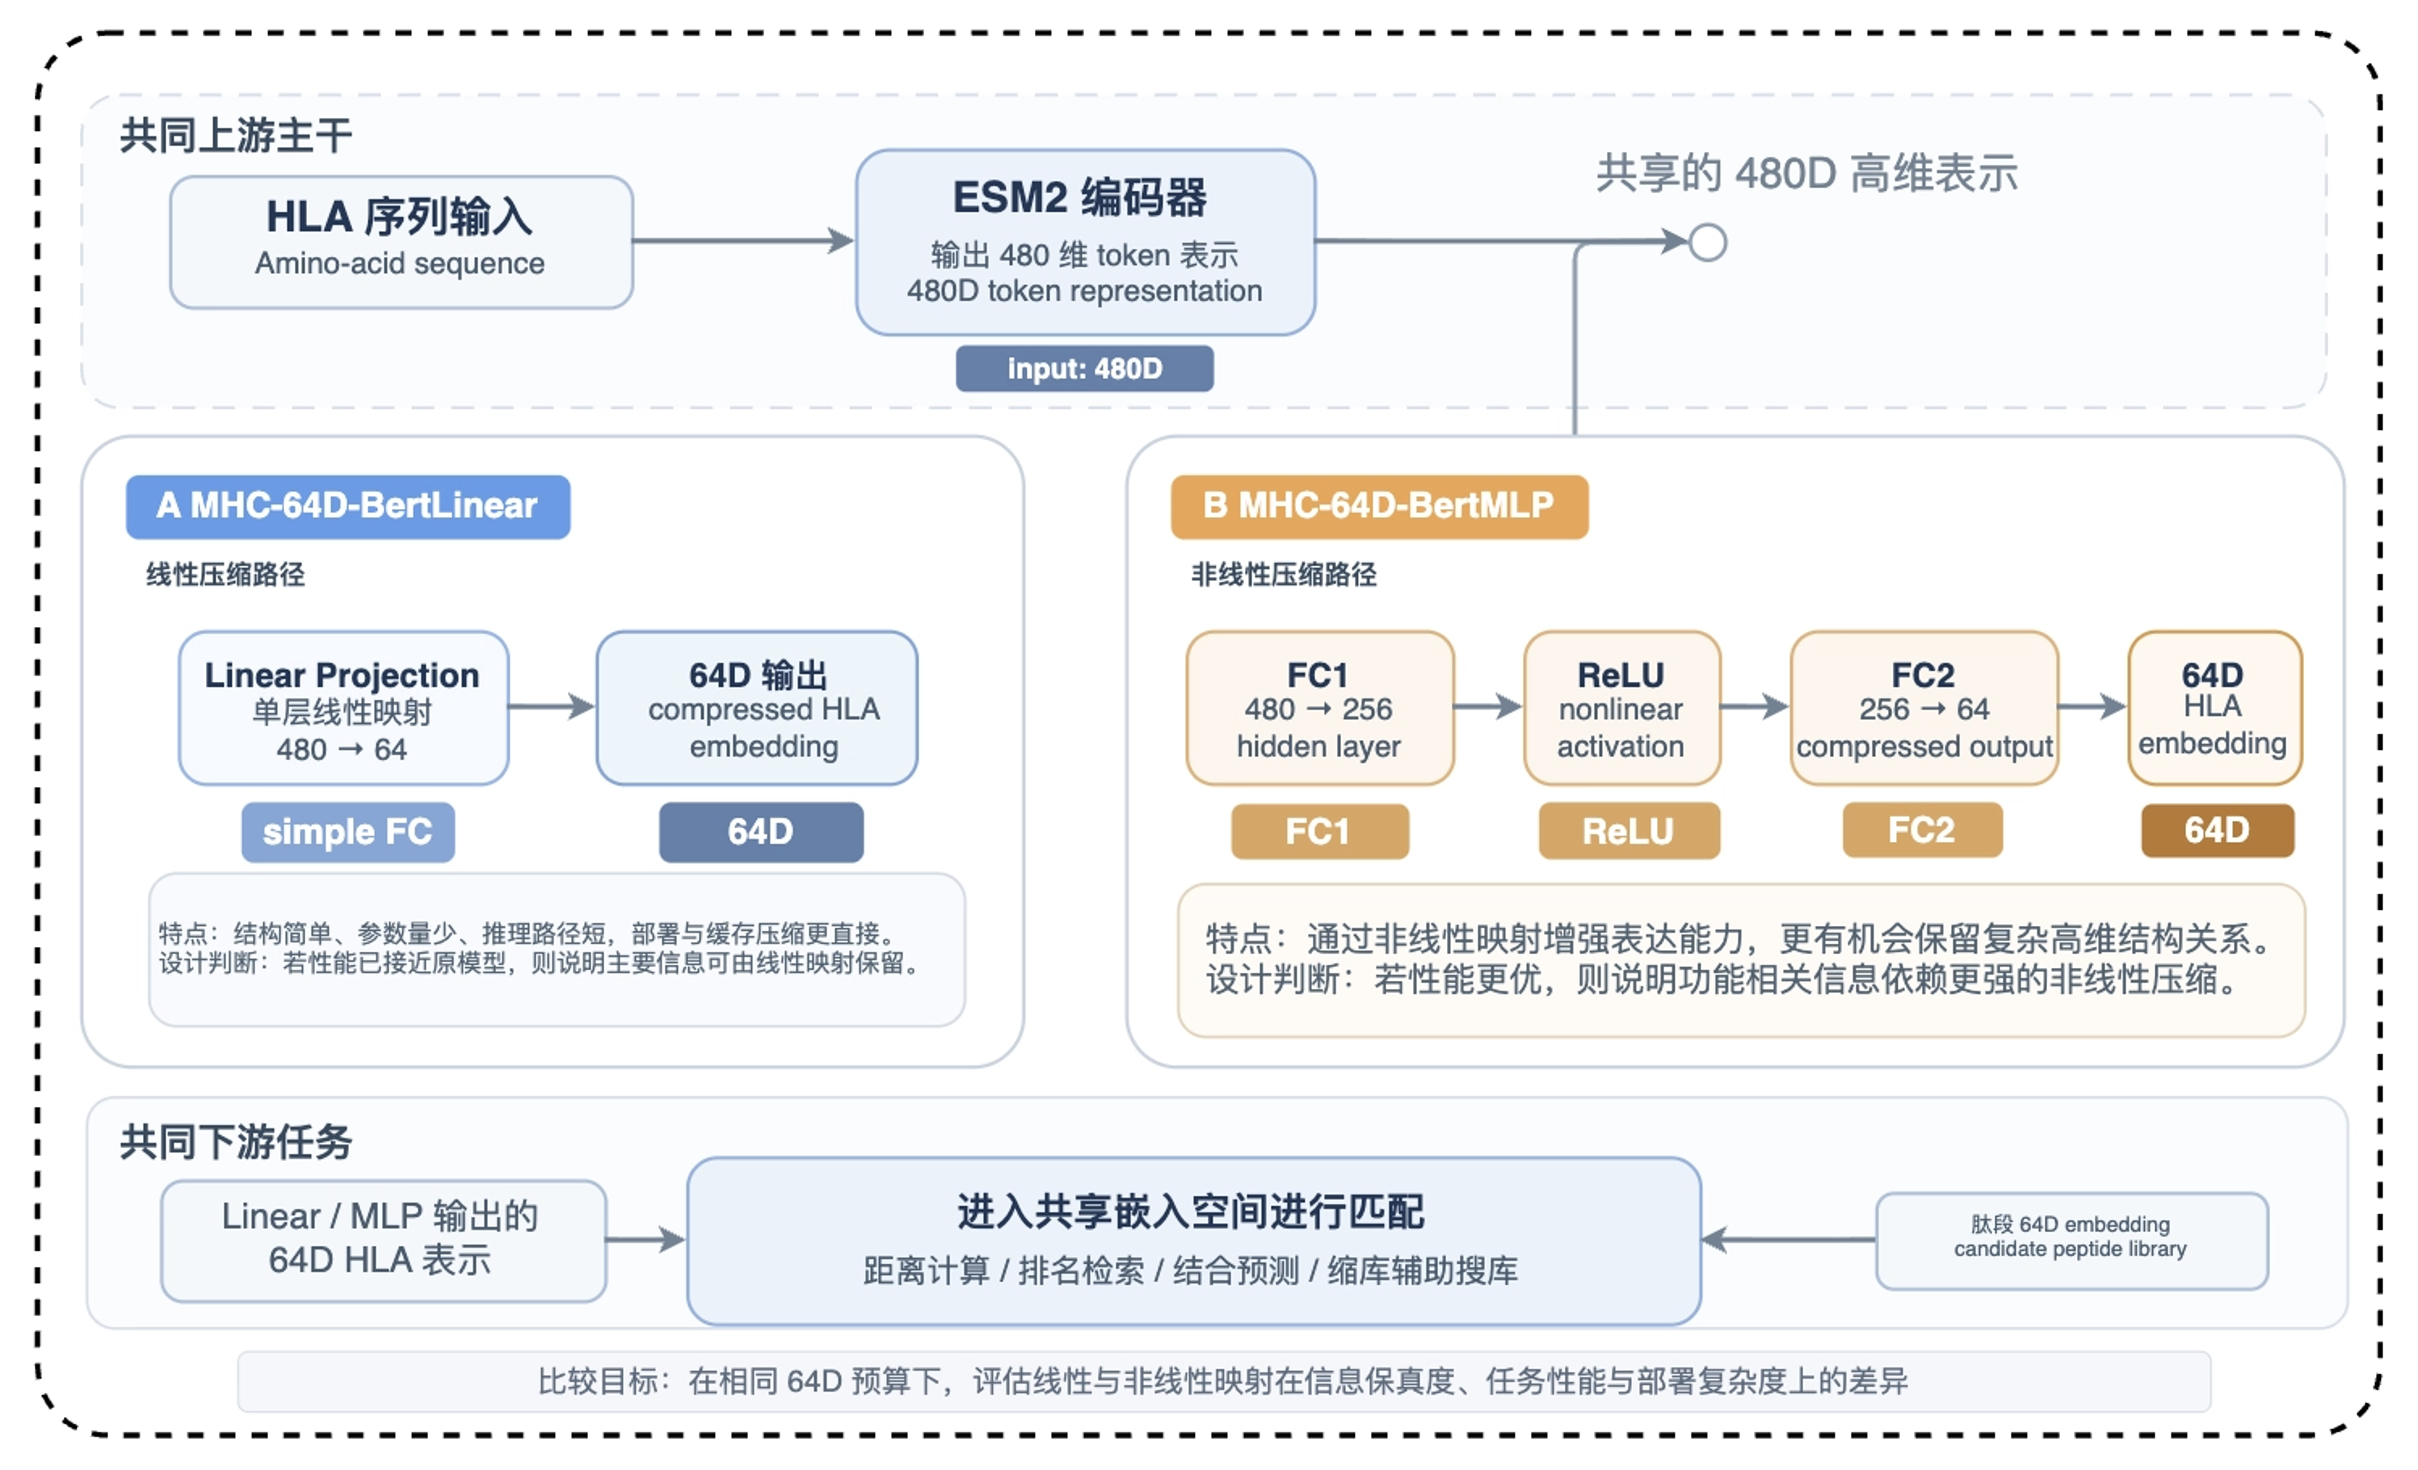
\includegraphics[width=1.0\textwidth]{figures/fig5_linear_mlp.png}
    \caption{Linear 与 MLP 的结构对比图}
    \label{fig:linear-mlp-structure}
\end{figure}

在该任务中，模型先根据目标 HLA 对候选肽段进行筛选，构建等位基因特异的缩减数据库；随后将这一缩库结果与直接检索流程进行比较。通过分析两种流程在肽段层面的 overlap，可以评价模型辅助缩库在压缩候选空间的同时能否有效保留基线检索结果。

本文采用 Precision-like、Recall-like、Overlap-F1、Loss Rate、Expansion Rate 和 Comprehensive Score 等指标，从覆盖度、一致性、结果丢失及新增差异等角度评价缩库效果。将 Linear 与 MLP 两类模型嵌入相同的下游流程进行比较，能够进一步判断不同降维结构在真实应用场景中的适用程度。

最终默认降维模型的选定需要综合多重因素，而不能仅依赖单一指标。本文主要从以下三个方面加以判断。

第一，常规预测性能。模型应在 rank-recall 和 distance-recall 上保持相对稳定，说明其候选排序能力和空间结构保持能力未受到明显冲击。第二，下游任务表现。模型应在缩库辅助搜库任务中保持较好的结果覆盖度和一致性，表明其不仅在测试指标上有效，也能在实际应用流程中发挥作用。第三，工程部署成本。若两类模型的性能差别不大，则结构更轻量、参数更少、实现成本更低的方案更适合作为默认部署模型。

因此，本文将于第三章结合常规预测指标与下游缩库辅助搜库结果，对 Linear 与 MLP 两类降维模型进行全面比较，并确定后续系统优化所采用的默认模型。

\subsection{基于重要性分析的结构剪枝}

在表示降维之后，我们从模型结构层面继续探索轻量化的空间。与输出降维主要降低缓存和距离计算成本不同，结构剪枝直接作用于模型内部网络，旨在削减编码器推理时的冗余计算。

FennOmix.MHC 的编码器采用了 Transformer 结构，其中的注意力头和前馈网络单元对最终表示的贡献并不均等，因此我们将剪枝目标聚焦于 attention head 和 Feed-forward Network（FFN）隐藏单元，通过分析它们的贡献来识别冗余部分。

我们的剪枝思路是：在训练或评估阶段收集各组件激活或梯度的信息，据此计算重要性指标并排序，随后移除低重要性组件，再通过实验检验剪枝后的性能保持情况。

为了判断哪些组件可以安全移除，需要为注意力头和前馈网络单元建立可比较的重要性指标。我们采用基于激活和梯度的分析方法，来衡量不同组件对模型输出的贡献。

对于注意力头，可以统计其输出激活的范数或与损失相关的梯度范数；如果在多个批次中某个注意力头持续表现出较低的激活或梯度，则意味着它的贡献可能较弱。前馈网络隐藏单元也可通过类似的激活强度或梯度响应来估计重要性。

不同层的数值尺度可能不同，因此需要对重要性分数进行归一化。我们可以在层内或全模型范围内进行组件得分比较，以避免单层数值整体偏高或偏低带来的干扰。得分较高的组件视为关键结构予以保留，得分较低且稳定的则作为候选剪枝对象。

这样，剪枝就不再是盲目的结构删除，而是依据贡献差异进行选择性压缩，有助于降低性能损失的风险。

在具体实现上，我们采用基于重要性排序的结构压缩。首先，用验证集或测试集对模型进行前向传播和必要的梯度计算，收集注意力头和前馈网络单元的激活或梯度信息；然后，对重要性分数进行累积和归一化，得到综合排序结果。

对于注意力头，根据重要性分数选出低贡献的 head，可以通过置零权重、屏蔽输出或结构性移除等方式来降低其影响。对于前馈网络单元，则按隐藏单元的重要性分数确定剪枝位置，移除低贡献单元或缩减中间层维度。

剪枝后，需要验证模型性能是否明显下降。我们从预测能力和部署收益两个维度来评价剪枝效果。

预测能力方面，剪枝后的模型仍需通过 rank-recall 和 distance-recall 等指标来测试，以判断候选排序能力和嵌入空间结构是否受损。如果表现保持稳定，则说明被移除的组件大概率是冗余的。

部署收益方面，关注剪枝对参数规模、计算量和推理效率的影响。结构化剪枝若能真正减少矩阵计算规模，就有可能降低推理延迟和资源占用；掩码式剪枝可以论证冗余的存在，但实际加速效果还需要结合具体实现来评估。

因此，剪枝实验不仅是为了观察性能变化，更在于验证模型内部存在可压缩的冗余，为后续更细粒度的结构优化提供依据。具体的剪枝结果和性能对比将在第三章给出。

\begin{figure}[htbp]
    \centering
    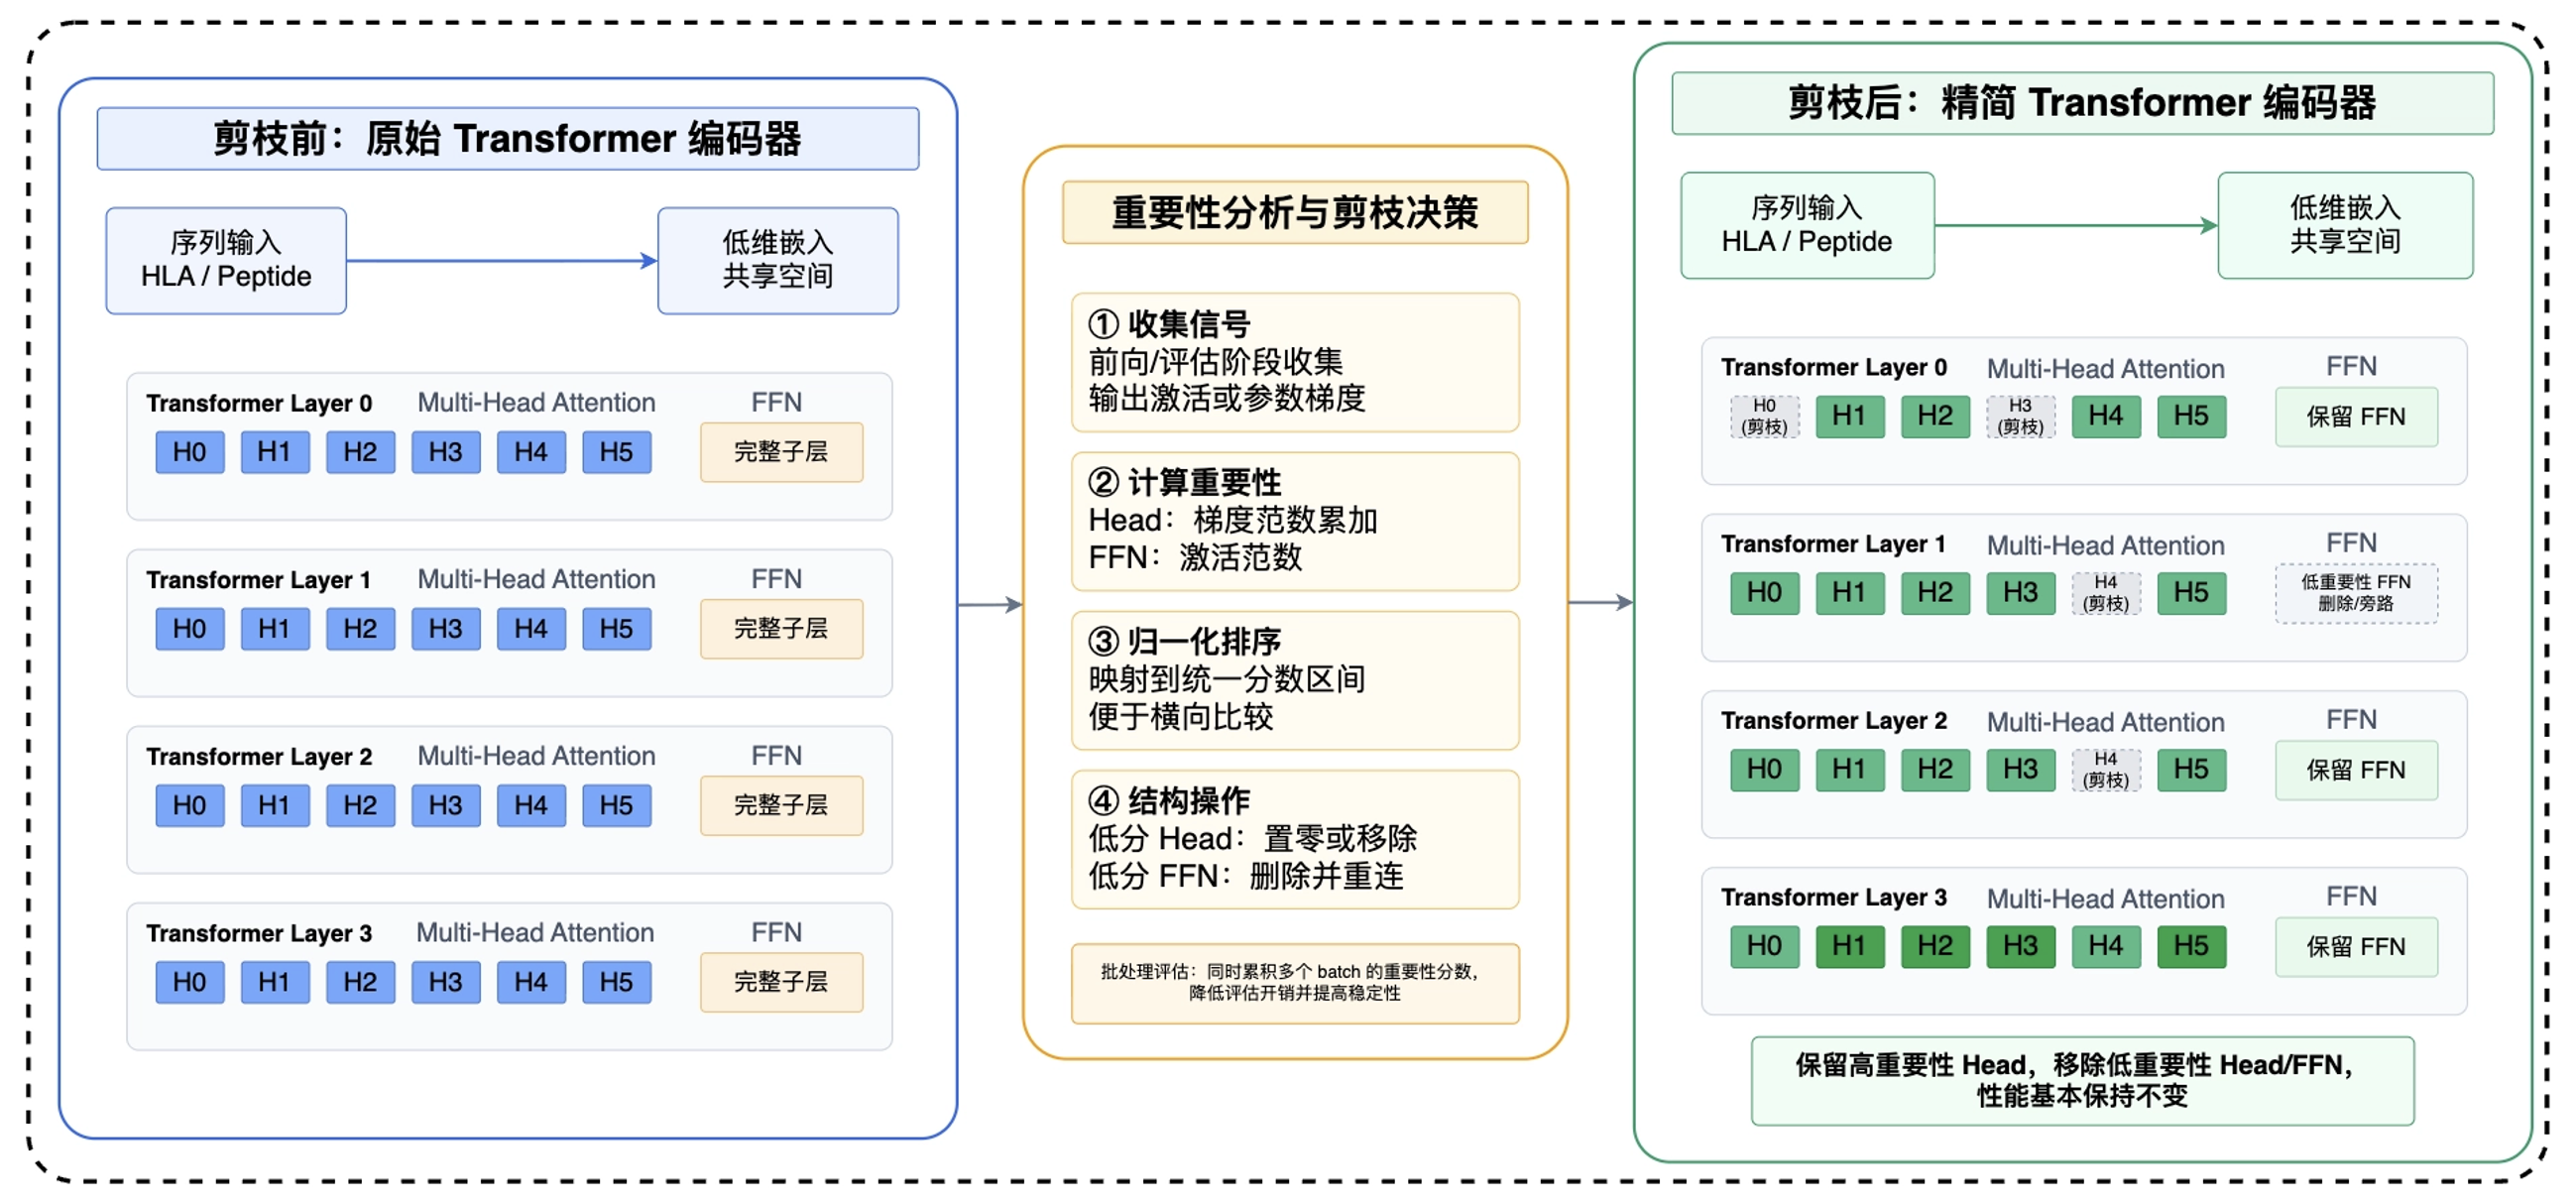
\includegraphics[width=1.0\textwidth]{figures/fig6_pruning_structure.png}
    \caption{剪枝前后结构示意图}
    \label{fig:pruning-structure}
\end{figure}

\section{肽段缓存压缩与索引机制设计}

\subsection{大规模肽段缓存问题}

在大规模候选肽段筛选与检索中，如果每次查询都实时调用肽段编码器重新生成 embedding，计算开销会非常大，系统响应速度也会明显下降。因此，预先对常见肽段进行批量编码并离线缓存，是支撑快速检索的关键前提。

借助缓存，在线阶段可以直接复用已有的肽段向量，只需对目标 HLA 或少量缓存外肽段实时编码，从而大幅减少重复推理。对于候选肽段规模庞大的场景，离线预计算与在线复用相结合，是提升可部署性和查询效率的重要方式。

然而，缓存在加速的同时也带来了新的系统问题。在大规模人类蛋白质组场景中，即便已经通过模型降维压缩了肽段 embedding 的维度，如果仍以 float32 精度存储，缓存体积依然偏大，会继续加重磁盘占用、内存加载和数据读取的负担。因此，在输出维度压缩后，仍有必要对缓存的表示方式和访问组织做进一步优化。

从系统设计看，肽段缓存主要面临两对矛盾。

第一，存储成本与表示精度相互制约。更高精度的浮点表示能更完整地保留模型输出，但存储体积也随之膨胀。若将所有肽段 embedding 以 float32 原样存储，缓存文件不仅占空间，也不利于跨环境传输、版本管理和长期归档。因此，需要在确保向量近似精度的前提下，引入更紧凑的数据表示。

第二，访问效率与资源占用彼此掣肘。将缓存向量一次性全部加载到内存，查询速度快，但内存压力也大；始终保留在磁盘中按需读取，虽然减轻了常驻内存负担，但在高频查询时容易受到 I/O 延迟的影响。这就需要系统根据不同场景设计灵活的加载策略，在访问效率和资源消耗之间找到平衡。

基于上述问题，我们从两个层面设计缓存机制：一方面，对低维肽段向量进一步采用 INT8 量化压缩来缩减缓存文件体积；另一方面，围绕缓存文件建立肽段索引，并设计全量加载和延迟加载两种访问模式，以适配不同的查询频率和资源条件。

\subsection{基于INT8的缓存量化压缩}

肽段缓存压缩的核心诉求并不是一味追求最小体积，而是在尽可能保持 embedding 表示精度的前提下，减少缓存的存储和传输开销。后续肽段向量还要与目标 HLA 嵌入进行距离计算，过大的压缩误差可能影响候选筛选的可靠性。因此，缓存压缩方法需要在压缩率、数值误差和实现复杂度之间取得平衡。

我们采用基于线性量化的对称 INT8 压缩方案，将原始 float32 向量映射为 INT8 表示。该方法的优点是压缩与反压缩计算简单，适合大规模批量处理；逐维缩放因子保留了各维度的数值尺度信息，有助于减小因维度分布差异带来的误差。

记肽段编码器输出的原始向量矩阵为 $X \in \mathbb{R}^{N \times D}$ ，其中，$N$ 为肽段总数，$D$ 为 embedding 维度，$x_{ij}$ 表示第 $i$ 条肽段在第 $j$ 维上的浮点值。

对每个维度 $j$，首先统计其均值和标准差：
\[
    \mu_j
    =
    \frac{1}{N}
    \sum_{i=1}^{N} x_{ij},
\]

\[
    \sigma_j
    =
    \sqrt{
        \frac{1}{N}
        \sum_{i=1}^{N}
        \left(x_{ij}-\mu_j\right)^2
    }
\]
为减轻极端值对量化范围的影响，本文采用基于 $k\sigma$ 的截断策略确定各维度的对称量化范围。令： $a_j = k\sigma_j$ ，由此，第 $j$ 维的量化区间为： $\left[-a_j, a_j\right]$ ，在此基础上，第 $j$ 维的缩放因子、截断值和量化整数可统一表示为： $s_j = \frac{a_j}{127}$ ，其中，127 对应 INT8 有符号整数正向范围的最大值。

为避免溢出，量化前先对原始浮点值进行截断：
\[
    \hat{x}_{ij}
    =
    \mathrm{clip}
    \left(
        x_{ij},
        -a_j,
        a_j
    \right)
\]
随后，利用缩放因子将浮点值映射为整数：
\[
    q_{ij}
    =
    \mathrm{round}
    \left(
        \frac{\hat{x}_{ij}}{s_j}
    \right)
\]
其中： $q_{ij} \in \left[-127,127\right]$ 。

量化后的 $q_{ij}$ 以 INT8 类型保存。对整个肽段向量矩阵而言，量化后的整数矩阵可表示为： $Q \in \mathbb{Z}^{N \times D}$ 。

在实际使用时，系统读取量化后的整数值 $q_{ij}$ 及对应维度的缩放因子 $s_j$，通过反量化即可恢复浮点近似值： $\widetilde{x}_{ij} = q_{ij} \cdot s_j$ 。

于是，原始 float32 向量便可表示为“INT8 数据块 + 逐维缩放因子”的组合，前者承载压缩后的主体数据，后者用于复原数值尺度。

量化误差可表示为原始浮点值与反量化近似值之差： $e_{ij} = x_{ij} - \widetilde{x}_{ij}$ 。

在不计截断误差的理想情形下，线性量化将连续区间划分为固定步长的离散取值，由四舍五入引起的单元素误差上界近似满足： $\left|e_{ij}\right| \le \frac{s_j}{2}$ 。

由上式可知，量化误差主要受缩放因子 $s_j$ 控制。缩放因子越小，离散化步长越细，量化误差越低；缩放因子越大，量化范围虽宽，但单个取值间隔也相应增大。因此，在设定量化范围时，应避免极端值过度拉大 $a_j$，否则会损害大部分样本的量化精度。

本文采用逐维独立量化，而非对所有维度使用统一缩放因子，原因在于不同 embedding 维度的数值分布可能存在差异，逐维缩放能更好地适配各维度的尺度变化，从而压低量化误差。后续第三章将通过实验统计量化前后的误差，并分析该压缩方法对缓存存储和向量表示的影响。

从存储角度看，float32 数据每个元素占 4 字节，INT8 每个元素占 1 字节。因此，在忽略少量缩放因子与文件头开销的情况下，向量主体数据体积可近似压缩至原来的四分之一，这为大规模肽段缓存的落盘、加载和传输提供了更紧凑的数据基础。

\subsection{自定义二进制缓存格式}

仅靠量化方法尚不足以构成完整的缓存机制，还需配合一种适宜批量存储与按索引访问的数据组织格式。若继续采纳文本格式或逐条对象序列化方式保存向量，不但会引入显著的额外开销，也不利于后续的随机访问和高效读取。有鉴于此，本文在量化之后进一步设计了自定义二进制缓存格式，用以组织大规模肽段向量数据。

与通用序列化方式相比，自定义二进制格式更契合本文的数据特征：向量维度固定、肽段数量庞大，且查询模式以按索引定位为主。针对这种“定长向量 + 大规模顺序块”的结构，紧凑的二进制布局能有效削减冗余元数据，并提升基于偏移量的读取效率。

本文设计的自定义二进制缓存文件主要由文件头、缩放因子区、量化数据区和肽段序列区构成，各部分功能如表~\ref{tab:binary-cache-format} 所示。

文件头赋予缓存文件自描述能力：系统读取文件头即可校验格式、版本，并获取肽段数量与向量维度等元信息。缩放因子区存放各维度对应的浮点缩放因子，供反量化时还原近似浮点向量。向量数据区以连续块形式保存所有肽段的 INT8 向量，使得系统能够按索引位置直接计算偏移量并读取对应的压缩数据。肽段序列区则记录各向量对应的原始肽段字符串，为后续哈希索引的构建提供基础。

自定义二进制格式并非孤立设计，而是与后续索引机制紧密衔接。由于所有量化向量按固定维度顺序连续存放，一旦获知某肽段对应的索引编号，即可直接计算出其在量化数据区中的偏移量。

设每个量化向量的维度为 $D$，每个 INT8 元素占 1 字节，第 $i$ 个肽段向量在数据区中的起始偏移量为：
\[
    \mathrm{offset}_i
    =
    \mathrm{offset}_{\mathrm{data}}
    +
    i \times D
\]
其中，$\mathrm{offset}_{\mathrm{data}}$ 为量化数据区的起始位置。通过该偏移量，系统可直接定位并读取第 $i$ 个肽段的压缩向量。

\begin{table}[htbp]
    \centering
    \caption{自定义二进制缓存文件结构}
    \label{tab:binary-cache-format}
    \begin{tabular}{p{0.18\textwidth} p{0.36\textwidth} p{0.36\textwidth}}
        \toprule
        区域 & 内容 & 作用 \\
        \midrule
        文件头
        & magic、version、肽段数量 $N$、向量维度 $D$、数据类型等
        & 标识文件格式，记录基础元数据 \\

        缩放因子区
        & 每个维度对应的缩放因子 $s_j$
        & 用于 INT8 向量反量化 \\

        向量数据区
        & 连续存储的 INT8 向量块
        & 保存压缩后的肽段 embedding \\

        肽段序列区
        & 肽段字符串列表或偏移表
        & 支持索引构建和查询定位 \\
        \bottomrule
    \end{tabular}
\end{table}

由此可见，二进制缓存格式为“按索引随机访问向量”提供了底层数据支撑，而索引模块则负责完成从“肽段字符串”到“向量位置”的映射。两者协同后，系统便能在在线查询阶段迅速判断缓存是否命中并读取对应向量。

\subsection{肽段哈希索引与加载策略}

完成缓存压缩后，系统还需应对另一关键问题：面对任意输入肽段，如何快速判断其是否已存于缓存，并在命中时即刻定位相应的嵌入向量。

为此，本文设计了基于“预计算缓存 + 字典查找”的肽段索引策略。其核心思路是将大规模候选肽段的编码工作前移至离线阶段，在线阶段则借助索引结构快速定位缓存向量。这样一来，系统在线阶段的主要任务便从“重复编码 + 遍历搜索”转化为“索引定位 + 向量读取”，从而有效缩短响应时间。

该策略尤其适合候选库规模庞大的场景。若在在线查询时逐条比对或重新编码，将很难满足响应需求。通过预计算缓存与索引查找，可以充分复用离线计算结果，显著提升常见肽段的查询效率。

索引结构定义为一个字典映射：
\[
    \mathrm{peptide\_index}
    :
    \mathrm{Dict}
    \left[
        \mathrm{str},
        \mathrm{int}
    \right]
\]
其中，索引以肽段序列字符串为键，对应的值是该肽段向量在缓存文件中的位置编号。在线查询时，系统会在 peptide\_index 中查找输入肽段：命中则直接返回位置编号，未命中则转入实时编码流程。

这种设计的查询效率很高。哈希字典的平均键值查找复杂度接近 $O(1)$，无需遍历全部候选肽段就能快速完成序列到缓存位置的定位。

从实现角度，索引必须与缓存文件严格保持同步。一旦缓存文件重新生成、肽段顺序调整或模型版本变更，索引也需要随之更新，否则可能出现位置与向量数据错位，影响查询准确性。

\begin{figure}[htbp]
    \centering
    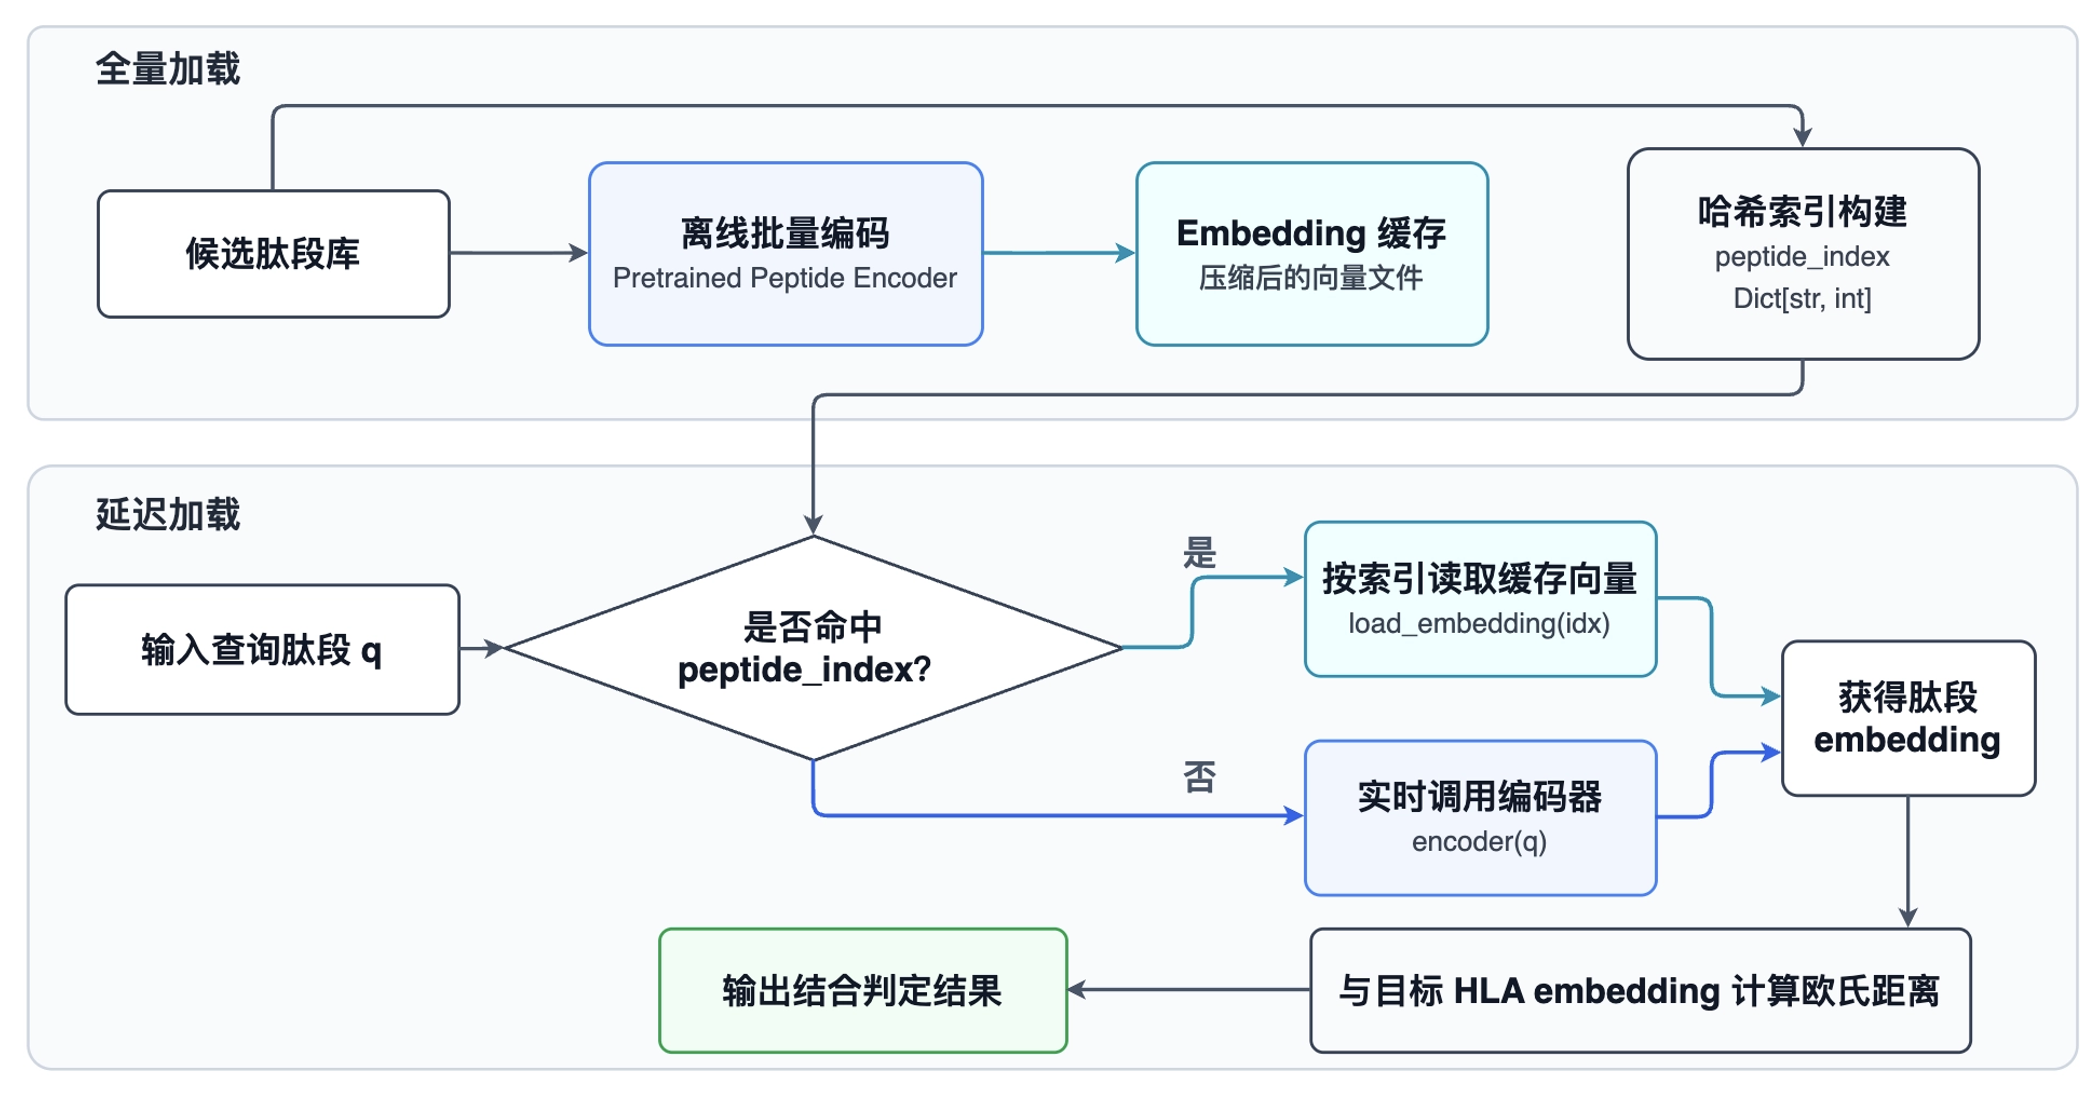
\includegraphics[width=1.0\textwidth]{figures/loading_strategy.png}
    \caption{全量加载与延迟加载结构图}
    \label{fig:loading-strategy}
\end{figure}

为了在访问速度和资源占用之间取得平衡，我们设计了两种加载模式：全量加载和延迟加载。

全量加载模式在系统启动时就把所有缓存向量读入内存。查询命中索引后，可以直接从内存数组中取出向量，访问速度很快，适合高频查询、批量筛选或内存充裕的服务器场景，但会占用较多的常驻内存。

延迟加载模式只在启动时加载肽段列表和索引结构，不立即载入全部向量。当某个肽段命中索引后，再根据其位置从磁盘缓存文件中读取向量。这种方式适合查询量不大或内存紧张的环境，能降低常驻内存压力，但在高频随机访问时容易受磁盘 I/O 制约。两种模式的实际资源收益将在第三章实验分析和第四章部署分析中详细说明。

\subsection{在线查询与匹配执行流程}

\begin{figure}[htbp]
    \centering
    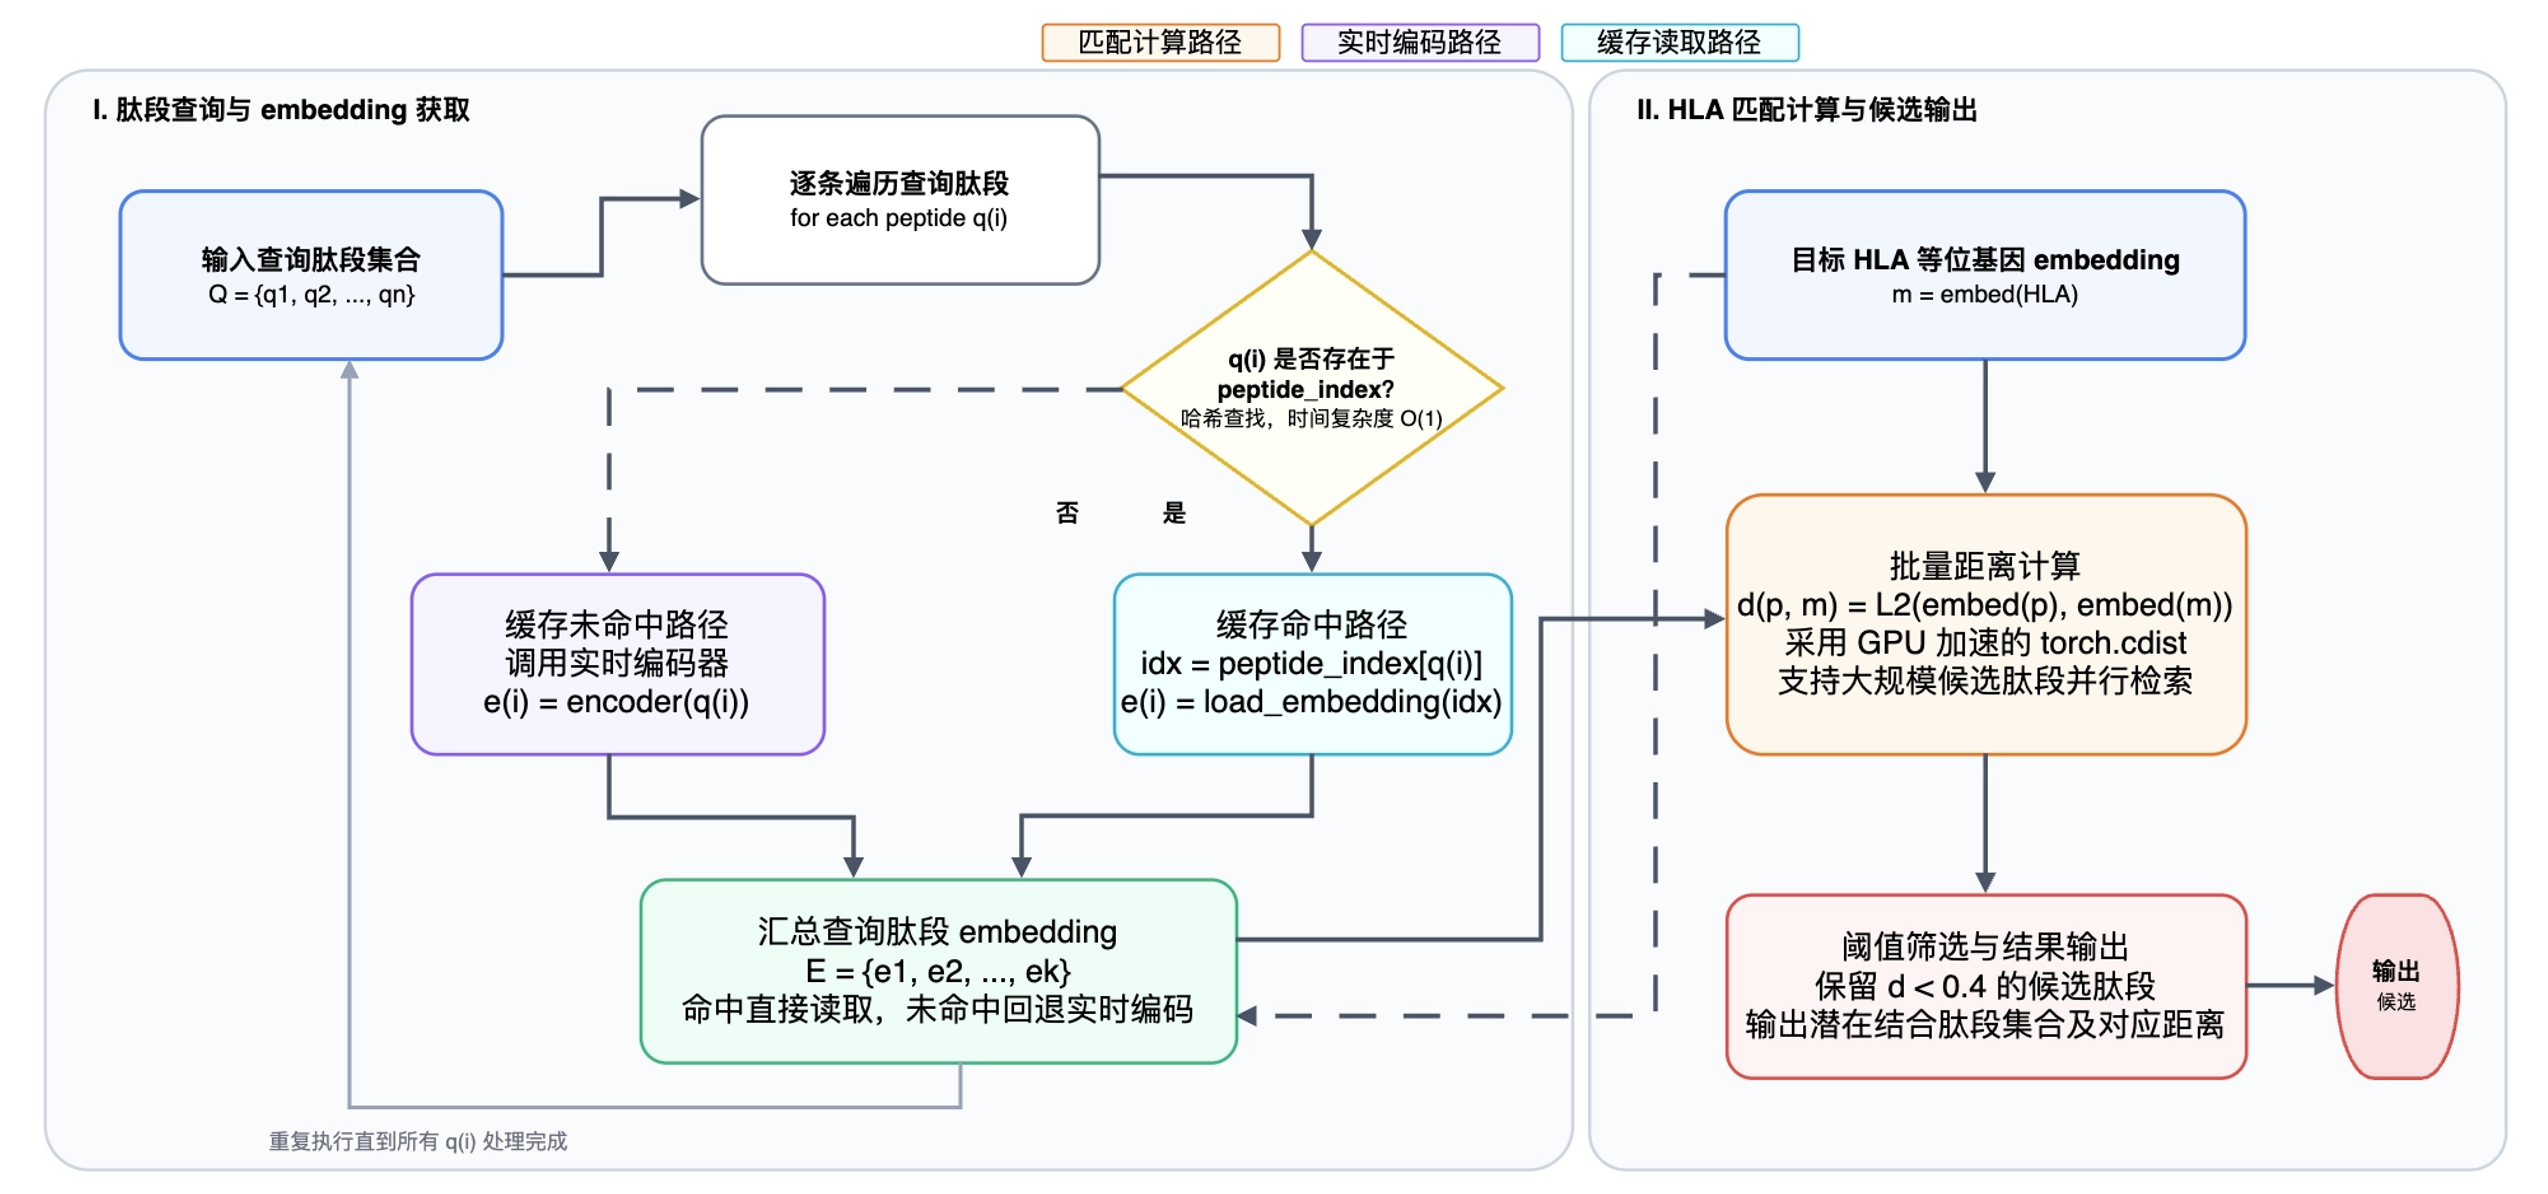
\includegraphics[width=1.0\textwidth]{figures/query_flow.png}
    \caption{完整查询流程图}
    \label{fig:query-flow}
\end{figure}

设输入查询肽段集合为 $Q = \left(q_1, q_2, \ldots, q_n\right)$，输出为对应的 embedding 集合 $E = \left(e_1, e_2, \ldots, e_n\right)$。

对每个查询肽段 $q_i$，系统先判断它是否在 \textit{peptide\_index} 中：如果在，就读取对应的缓存向量；如果不在，则调用肽段编码器实时生成 embedding。这样既复用了缓存，也保留了对新肽段的开放处理能力。

% 查询肽段向量获取流程的伪代码如下：

% \begin{tcolorbox}[
%     breakable,
%     enhanced,
%     colback=white,
%     colframe=black,
%     boxrule=0.5pt,
%     arc=0pt,
%     width=0.90\textwidth,
%     center,
%     left=6pt,
%     right=6pt,
%     top=6pt,
%     bottom=6pt
% ]
%     \ttfamily
%     输入：查询肽段集合 $Q$，肽段索引 peptide\_index，缓存文件 cache，肽段编码器 encoder\\
%     输出：肽段向量集合 $E$\\[0.5em]

%     E = []\\
%     for q in Q:\\
%     \hspace*{2em}if q in peptide\_index:\\
%     \hspace*{4em}idx = peptide\_index[q]\\
%     \hspace*{4em}e = load\_embedding(cache, idx)\\
%     \hspace*{2em}else:\\
%     \hspace*{4em}e = encoder(q)\\
%     \hspace*{2em}E.append(e)\\[0.5em]
%     return E
% \end{tcolorbox}

这一流程的好处在于，已缓存的肽段可以直接复用离线计算结果，避免重复编码；而缓存未覆盖的肽段则通过实时编码来处理。因此，系统既能从高缓存命中率中获益，又不会受限于固定的候选库。

拿到肽段 embedding 之后，系统需要进一步评估它们与目标 HLA 的结合可能性。这一步通过计算肽段嵌入与目标 HLA 嵌入之间的距离来完成：距离越小，两者在共享嵌入空间中越靠近，肽段成为潜在结合候选的概率就越高。

设目标 HLA 的嵌入向量为 $h$，某个肽段的嵌入向量为 $e_i$，两者之间的欧氏距离为 $d_i = \left\| h - e_i \right\|_2$。对于一组候选肽段，可以得到距离集合 $D_Q = \left\{d_1, d_2, \ldots, d_n\right\}$。

系统可以根据距离阈值或排序结果来筛选潜在结合肽段，比如选出距离小于某阈值的肽段，或按距离升序排列后取排名靠前的部分。实际实现中，可以采用批量矩阵计算来提升距离计算的效率。

这与 FennOmix.MHC 共享嵌入空间的设计思路是一致的：缓存模块解决向量存储与读取，索引模块解决快速定位，距离计算模块完成最终的匹配判断。

整体来看，我们设计的查询链路可以概括为：查询输入 $\rightarrow$ 哈希索引判定 $\rightarrow$ 命中则读缓存 / 未命中则实时编码 $\rightarrow$ 批量距离计算 $\rightarrow$ 输出潜在结合肽段。

这条链路的特点在于将离线缓存与在线编码无缝融合：一方面充分利用预计算缓存来提升常见肽段的查询效率，另一方面保留实时编码路径以处理新出现的肽段。缓存压缩、索引检索和距离匹配共同构成了面向在线预测的执行机制。

\section{本章小结}

本章梳理了实验和系统部署所需的理论与方法。我们从 MHC-I 抗原递呈、HLA 多态性和任务形式出发，明确了免疫多肽结合预测的生物学背景和计算目标，随后介绍了 FennOmix.MHC 的双模态编码、共享嵌入空间和对比学习思想，并给出了 rank-recall、distance-recall 以及缩库辅助搜库 overlap 分析等评价体系。

在方法设计上，本章针对大规模候选肽段场景下的部署瓶颈，采用了编码维度压缩、Linear 与 MLP 降维比较以及基于重要性分析的结构剪枝方法；同时，围绕肽段缓存体量大和访问效率受限的问题，设计了 INT8 量化压缩、自定义二进制缓存格式、哈希索引、全量与延迟加载策略以及完整的在线查询流程。这些内容共同构成了本文“理论基础—方法设计—系统优化”的核心框架，为第三章的实验验证和第四章的部署分析提供了基础。
